\documentclass[pdftex,twocolumn,epjc3]{svjour3}          % twocolumn

\RequirePackage[T1]{fontenc}

\smartqed  % flush right qed marks, e.g. at end of proof

\usepackage{graphicx,amstext,amsmath,amsfonts,mathptmx,epstopdf,subfigure,float,multirow,booktabs,bbm}
	
\RequirePackage[numbers,sort&compress]{natbib}
\RequirePackage[colorlinks,citecolor=blue,urlcolor=blue,linkcolor=blue]{hyperref}

%\journalname{Eur. Phys. J. C}

\begin{document}

%\title{Improved reversible data hiding based on PVO and adaptive pairwise embedding\thanks{This work was supported by the National Key Research and Development of China (No. 2016YFB0800404), the National Science Foundation of China (Nos. 61572052, U1736213, 61532005, 61332012), and the Fundamental Research Funds for the Central Universities (Nos. 2018JBZ001, 2017RC008).}}
%
%\author{Haorui Wu
%\and
%Xiaolong Li
%\and
%Yao Zhao
%\and
%Rongrong Ni
%}

\title{Improved reversible data hiding based on PVO and adaptive pairwise embedding
\thanksref{t1}
}

\author{Haorui Wu\thanksref{e1,addr1,addr2}
\and
Xiaolong Li\thanksref{e2,addr1,addr2} %etc.
\and
Yao Zhao\thanksref{e3,addr1,addr2}
\and
Rongrong Ni\thanksref{e4,addr1,addr2}
}

\thankstext[$\star$]{t1}{This work was supported by the National Key Research and Development of China (No. 2016YFB0800404), the National Science Foundation of China (Nos. 61572052, U1736213 and 61532005), and the Fundamental Research Funds for the Central Universities (No. 2018JBZ001).}
\thankstext{e1}{e-mail: hrwu@bjtu.edu.cn}
\thankstext{e2}{e-mail: lixl@bjtu.edu.cn}
\thankstext{e3}{e-mail: yzhao@bjtu.edu.cn}
\thankstext{e4}{e-mail: rrni@bjtu.edu.cn}

\institute{Institute of Information Science, Beijing Jiaotong University, Beijing 100044, China\label{addr1}
\and
Beijing Key Laboratory of Advanced Information Science and Network Technology, Beijing 100044, China\label{addr2}
}

\date{Received: October 2018}

\maketitle

\begin{abstract}
Pixel-value-ordering (PVO) is an efficient technique of reversible data hiding (RDH). By PVO, the cover image is first divided into non-overlapping blocks with equal size. Then, the pixel values in each block are sorted in ascending order. Next, take the second largest/samllest pixel value as a prediction of the largest/samllest pixel value to derive two prediction-errors. Finally, the data embedding is constructed by modifying the generated prediction-errors of each block. After data embedding, the PVO of each block is unchanged, which guarantees the reversibility. Our key observation is that, in each block, the modification for the two prediction-errors is independent without exploiting the correlation between them, although they are closely correlated to each other. In light of this, an improved PVO-based RDH method is proposed in this work. The two prediction-errors of each block is considered as a pair, and the pairs are modified for data embedding based on adaptive two-dimensional histogram modification. The proposed method is experimentally verified better than the original PVO-based method and some of its improvements.
\keywords{Reversible data hiding \and Pixel-value-ordering \and Two-dimensional histogram \and Pairwise embedding \and Adaptive embedding}
\end{abstract}

\section{Introduction}\label{intro}

Information hiding is a hot-spot of current information security studies \cite{
Cox2007Digital,
Fridrich2009Steganography,
Zhang2006Efficient,
Zhang2011Reference,
Qin2014Novel,
Qin2015Effective,
Hong2017Coherent,
Ma2019Selection}.
Among the numerous information hiding techniques,
reversible data hiding (RDH) is a special one. By RDH, the decoder can perfectly recover the cover image after extracting the embedded secret data. The key question of RDH is how to minimize the embedding distortion for a given embedded capacity.

So far, RDH has been widely studied and many effective reversible embedding methods have been proposed in
\cite{Tian2003Reversible(DE),
Ni2006Reversible(HS),
Thodi2007Expansion(PEE),
Hong2009Reversible(PEE),
Sachnev2009Reversible(PEE),
coatrieux2009reversible(adaptive),
Li2011Efficient(PEE),
Coltuc2011Improved(PEE),
Hong2011Adaptive(PEE),
Ou2013Pairwise(PEE),
Li2013A(DE),
Qin2013An(PEE),
Li2013General(HS),
xuan2013optimal(adaptive),
dragoi2014local,
qian2014reversible,
Li2015Efficient(PEE),
Pan2015Reversible(PEE),
dragoi2015local,
dragoi2016adaptive,
shi2016reversible,
wang2017rate(adaptive),
DBLP:journals/jrtip/KimYKY18,
DBLP:journals/jrtip/Jung18a,
Ou2018}.
Among the present RDH methods, the ones based on prediction-error expansion (PEE) have shown an outstanding performance by exploiting the correlations between adjacent pixels. The PEE technique is first proposed by Thodi and Rodriguez in \cite{Thodi2007Expansion(PEE)}. In this method, a prediction-error histogram is first generated, and then this histogram is modified to embed data based on expansion and shifting the histogram bins. Later on, the PEE technique has been widely adopted and developed in RDH studies. These developments are mainly based on, for example, sharper histogram generation with an accurate predictor design \cite{Sachnev2009Reversible(PEE),dragoi2014local,dragoi2015local}, adaptive histogram modification \cite{coatrieux2009reversible(adaptive),xuan2013optimal(adaptive),wang2017rate(adaptive)}, two-dimensional histogram modification \cite{Li2013A(DE),Ou2013Pairwise(PEE),dragoi2016adaptive}, and multiple histogram modification \cite{Li2015Efficient(PEE)}.

The pixel-value-ordering (PVO) based RDH is first proposed by Li \emph{et al.} in \cite{Li2013High(PVO)}. In this method, a new predictor is designed based on PVO for PEE. Specifically, the cover image is first divided into non-overlapping blocks with equal size, and, for each block, its pixel values are sorted in ascending order. Next, the second largest/samllest pixel value is taken as a prediction of the largest/samllest pixel value to derive two prediction-errors. Finally, the data embedding is conducted by modifying the generated prediction-errors of each block. After data embedding, the PVO of each block remains unchanged, which ensures the reversibility. The PVO-based prediction can derive an accurate predictor, and its performance is proved better than some other PEE-based methods, especially for low embedding capacities. Later on, the PVO-based method \cite{Li2013High(PVO)} has been improved in some works \cite{Peng2014Improved(PVO),Ou2014Reversible(PVO),qu2015pixel,wang2015novel,Ou2016High,He2018Reversible,Dragoi2018Improved} in many aspects.

In this paper, we try to improve the embedding performance of PVO-based RDH. Our key observation is that, for the PVO-based methods such as \cite{Li2013High(PVO)} and \cite{Peng2014Improved(PVO)}, in each divided image block, the modification for the two prediction-errors is independent without exploiting the correlation between them, although they are closely correlated to each other. In this work, the two prediction-errors of each block is considered as a pair, and the pairs are modified for data embedding based on two-dimensional (2D) histogram modification. The 2D histogram modification manner is adaptively determined in our work such that the embedding performance is optimized. Moreover, inspirited by \cite{Li2013High(PVO),Peng2014Improved(PVO)}, a block selection strategy is employed as well. Only the smooth image blocks are selected for data embedding while the rough ones are unmodified. The experimental results show that the performance of the proposed method is better than the original PVO-based RDH method \cite{Li2013High(PVO)} and some of its improvements \cite{Peng2014Improved(PVO),Ou2014Reversible(PVO)}.

The rest of the paper is arranged as follows. Section~\ref{Related Work} provides a brief review for two typical PVO-based methods \cite{Li2013High(PVO)} and \cite{Peng2014Improved(PVO)}. Section~\ref{Proposed Method} introduces the proposed PVO-based RDH. Experimental results are reported in Section~\ref{Experimental Results}. Finally, Section~\ref{Conclusion} concludes this paper.

\section{Related work} \label{Related Work}

In this section, as a preparation, the original PVO-based RDH method \cite{Li2013High(PVO)} and its improvement \cite{Peng2014Improved(PVO)} are reviewed.
\textcolor[rgb]{1.00,0.00,0.00}{Moreover, a recently proposed RDH method, pairwise PEE \cite{Ou2013Pairwise(PEE)}, is briefly introduced as well.}

\subsection{PVO-based RDH  \cite{Li2013High(PVO)}}

The PVO-based RDH technique is first proposed by Li \emph{et al.} in \cite{Li2013High(PVO)}. For this method, first, the cover image is divided into non-overlapping blocks sized $n_1 \times n_2$. Then, for a given block, sort its pixels $(p_1,...,p_n)$ in ascending order according to the pixel values to obtain $(p_{\sigma(1)},...,p_{\sigma(n)})$, where $\sigma: \{1,...,n\} \rightarrow \{1,...,n\}$ is the unique one-to-one mapping satisfying $\sigma(i) < \sigma(j)$ if $p_{\sigma(i)} = p_{\sigma(j)}$ and $i < j$, and $n = n_1 \times n_2$. Next, take the second largest pixel value $p_{\sigma(n-1)}$ as the prediction of the largest pixel value $p_{\sigma(n)}$, and define the prediction-error as
\begin{equation}\label{eq:1}
d_{\rm max} = p_{\sigma(n)} - p_{\sigma(n-1)}.		
\end{equation}		
Take the standard gray-scale Lena image with $2 \times 2$ sized blocks as an example, the histogram of prediction-error $d_{\rm max}$ is shown in Figure~\ref{fig:1}. It can be observed that the histogram is defined in the interval $[0,+\infty)$ since $d_{\rm max} \geq 0$, and it has a peak value at bin 1.
Then, based on this peak property of the generated histogram, $d_{\rm max}$ is modified according to the following rule to derive the marked prediction-error $\widetilde{d}_{\rm max}$ as
\begin{equation}\label{eq:2}
\widetilde{d}_{\rm max} = \left\{\begin{array}{ll}
d_{\rm max},    &   \text{if } d_{\rm max}=0 \\
d_{\rm max}+b,  &   \text{if } d_{\rm max}=1 \\
d_{\rm max}+1,  &   \text{if } d_{\rm max}>1
\end{array}\right.		
\end{equation}
where $b\in \{0,1\}$ is a to-be-embedded secret data bit. Finally, the largest pixel value $p_{\sigma(n)}$ is modified as
\begin{equation}\label{eq:ppp}
\widetilde{p}_{\sigma(n)} = p_{\sigma(n-1)} + \widetilde{d}_{\rm max}
\end{equation}
to derive the marked pixel value.

\begin{figure}
\centering
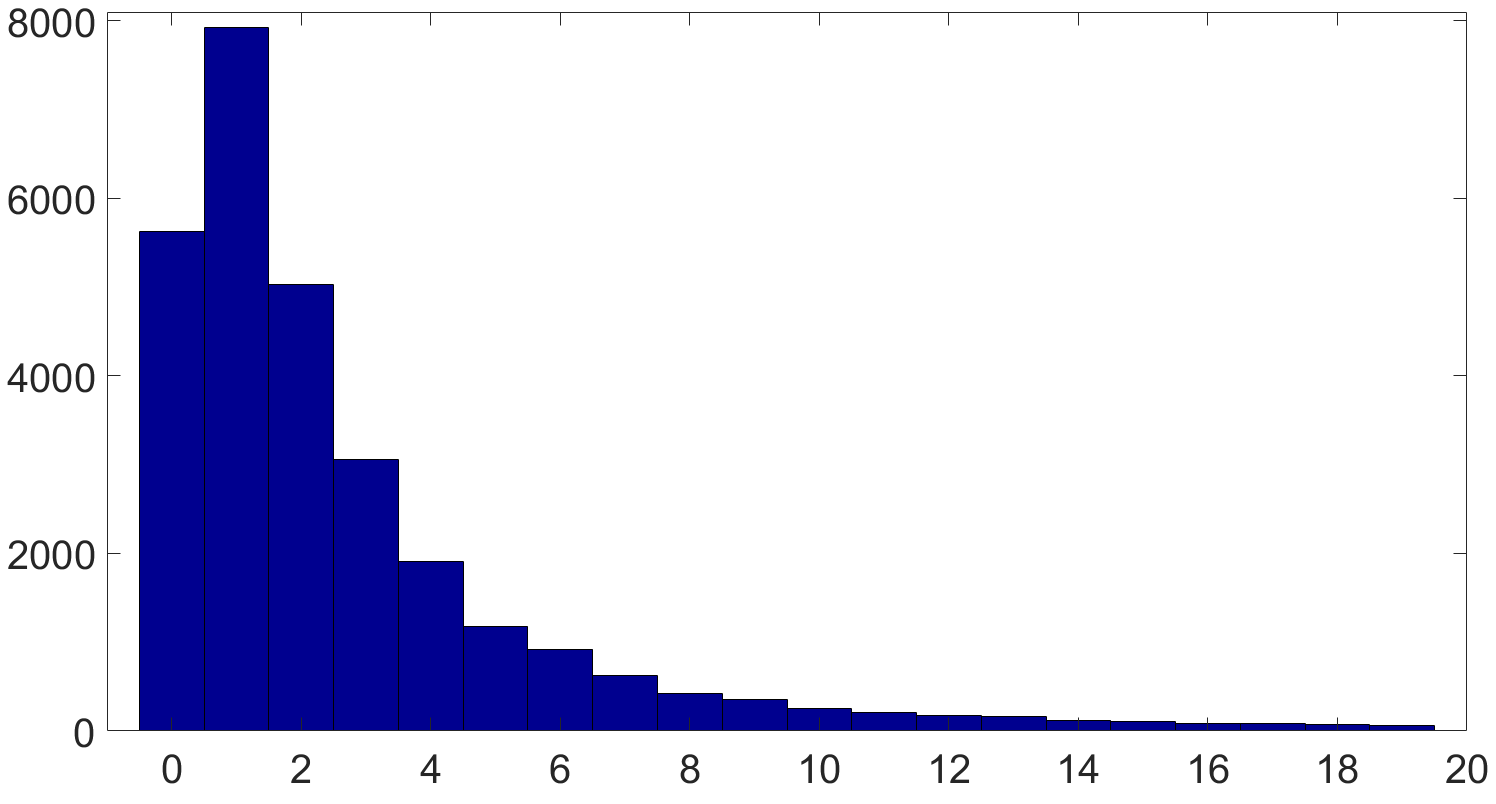
\includegraphics[width=0.4\textwidth]{./PVO_Lena_3x3.png}
\caption{Histogram of $d_{\rm max}$ defined in \eqref{eq:1}, for the standard $512 \times 512$ sized gray-scale image Lena with block size of $2 \times 2$.}
\label{fig:1}
\centering
\end{figure}

In the above procedure, for each block, only the largest pixel value with prediction-error larger than 0 maybe modified, in which this largest value is either unchanged or increased by 1 while other pixels remain unchanged. As a result, the PVO of each block is unchanged as well, and this property guarantees the reversibility. Specifically, for the decoder, the same as the data embedding process, the marked image is also divided into non-overlapping blocks of size $n_1 \times n_2$. Then, for a given block, sort its pixel values in ascending order to obtain $(\widetilde{p}_{\sigma(1)},...,\widetilde{p}_{\sigma(n)})$. Notice that $\widetilde{p}_{\sigma(i)} = p_{\sigma(i)}$ holds for each $1 \leq i \leq n-1$. Next, compute the marked prediction-error
\begin{equation}\label{eq:}
\widetilde{d}_{\rm max} = \widetilde{p}_{\sigma(n)} - \widetilde{p}_{\sigma(n-1)}.
\end{equation}
Finally, recover the original pixel value $p_{\sigma(n)}$ as
\begin{equation}\label{eq:4}
p_{\sigma(n)}=\left\{\begin{array}{ll}
\widetilde{p}_{\sigma(n)}, & \text{if } \widetilde{d}_{\rm max} \in \{0,1\}\\
\widetilde{p}_{\sigma(n)}-1, & \text{if } \widetilde{d}_{\rm max}>1
\end{array}\right.
\end{equation}
and extract the embedded data as $b = \widetilde{d}_{\rm max}-1$ in the case of $\widetilde{d}_{\rm max} \in \{1,2\}$. Moreover, since only the largest pixel value of each block maybe modified in the data embedding procedure, for each $1 \leq i \leq n-1$, $p_{\sigma(i)}$ can be recovered as $\widetilde{p}_{\sigma(i)}$ itself.

Furthermore, the smallest pixel value $p_{\sigma(1)}$ in each block can also be modified (either decreased by 1 or unchanged) to embed data. The similar data embedding and extraction procedures are omitted here.

\subsection{Improved PVO-based RDH \cite{Peng2014Improved(PVO)}} \label{IPVO}

In the original PVO-based RDH method, the blocks with $d_{\rm max} = 0$ are not utilized to carry data. However, these blocks are usually smooth and suitable for reversible embedding. Based on this consideration, in order to take the advantage of the blocks with $d_{\rm max} = 0$, an improved PVO-based method is proposed by Peng \emph{et al.} in \cite{Peng2014Improved(PVO)}.

For the data embedding of this method, first, for a given block with sorted values $(p_{\sigma(1)},...,p_{\sigma(n)})$, instead of computing the prediction-error $d_{\rm max}$ in \eqref{eq:1} as the original PVO-based method does, it is redefined as follows considering the order of $\sigma(n-1)$ and $\sigma(n)$
\begin{equation}\label{eq:5}
d_{\rm max}=\left\{\begin{matrix}
p_{\sigma(n)}-p_{\sigma(n-1)}, & \text{if } \sigma(n)>\sigma(n-1)\\
p_{\sigma(n-1)}-p_{\sigma(n)}, & \text{if } \sigma(n)< \sigma(n-1)
\end{matrix}\right..
\end{equation}
Clearly, one can verify that the redefined prediction-error satisfies $d_{\rm max} \geq 0$ if $\sigma(n)>\sigma(n-1)$, and $d_{\rm max} < 0$ if $\sigma(n)<\sigma(n-1)$. That is to say, the prediction-error defined in this way is ranged from $-\infty$ to $+\infty$. For example, for the Lena image, the histogram of the redefined prediction-error $d_{\rm max}$ is shown in Figure~\ref{fig:2}. This histogram is a Laplacian-like distribution centered at 0 with two sides decay. Then, the bins 0 and $-1$ are expanded for data embedding. More specifically, $d_{\rm max}$ is modified to derive the marked prediction-error $\widetilde{d}_{\rm max}$ in the following way
\begin{equation}\label{eq:6}
\widetilde{d}_{\rm max} = \left\{\begin{array}{ll}
d_{\rm max}+b, & \text{if } d_{\rm max}=0 \\
d_{\rm max}-b, & \text{if } d_{\rm max}=-1 \\
d_{\rm max}+1, & \text{if } d_{\rm max}\geq 1 \\
d_{\rm max}-1, & \text{if } d_{\rm max}\leq -2	
\end{array}\right.
\end{equation}
where $b\in \{0,1\}$ is a to-be-embedded data bit. Accordingly, the largest pixel value $p_{\sigma(n)}$ is modified as
\begin{equation}
\widetilde{p}_{\sigma(n)} = p_{\sigma(n-1)} + |\widetilde{d}_{\rm max}|
\end{equation}
to derive the marked pixel value.

For this improved method, a key issue is that, unlike other expansion-shifting based RDH methods, the expansion bins can not be arbitrarily selected. To guarantee the reversibility, the sign of each prediction-error (i.e., ``$\geq 0$'' or ``$<0$'') shouldn't be changed after data embedding.

\begin{figure}
\centering
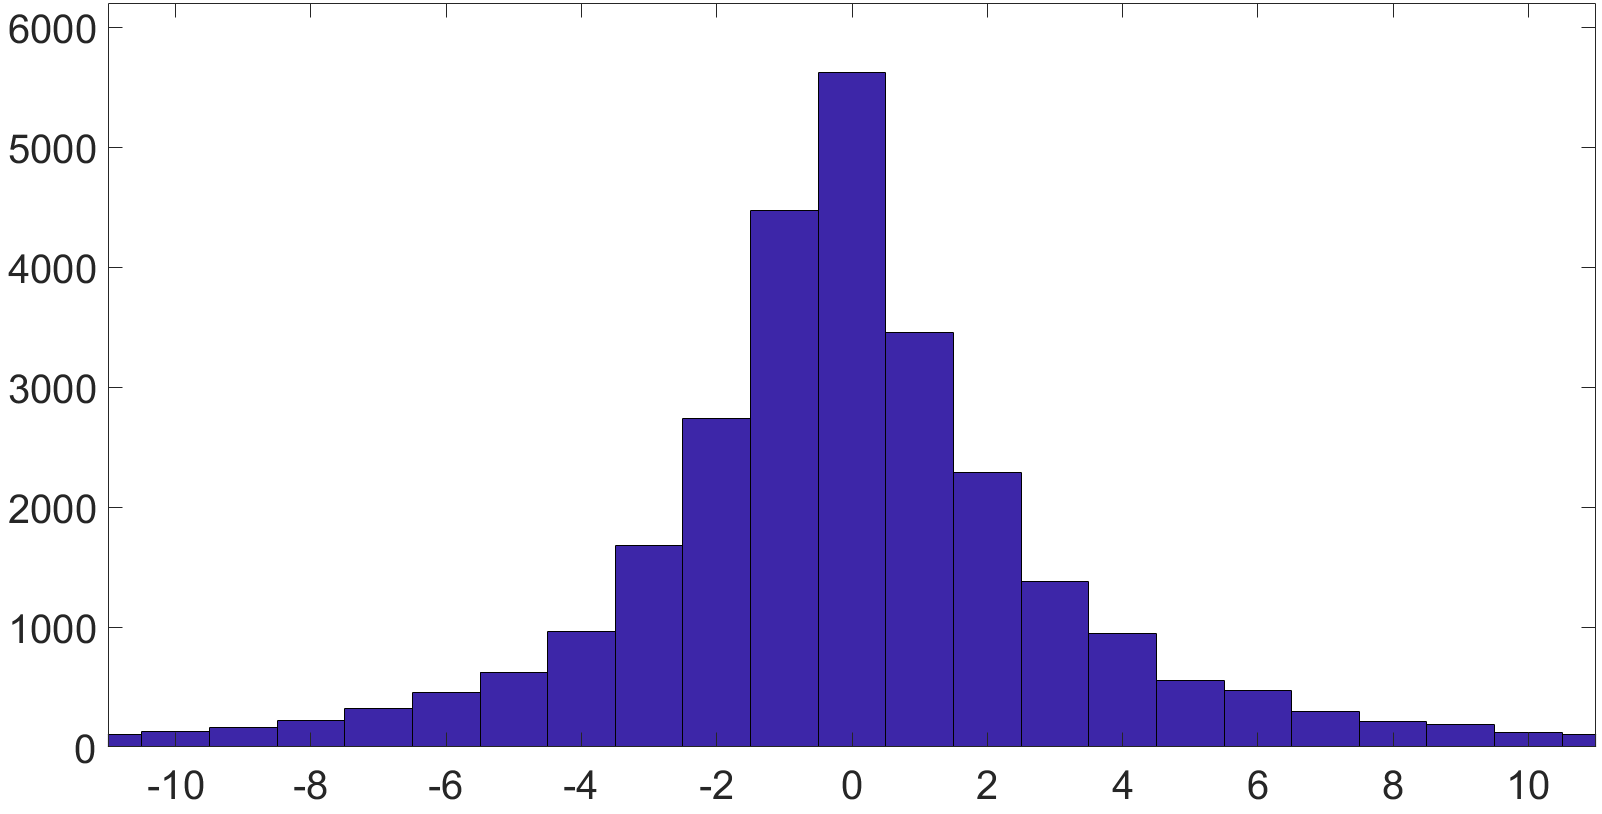
\includegraphics[width=0.4\textwidth]{./IPVO_Lena_3x3.png}
\caption{Histogram of $d_{\rm max}$ defined in \eqref{eq:5}, for the standard $512 \times 512$ sized gray-scale image Lena with block size of $2 \times 2$.}
\label{fig:2}       % Give a unique label
\centering			
\end{figure}

Similar with \cite{Li2013High(PVO)}, in each block, only the largest pixel value $p_{\sigma(n)}$ is either increased by 1 or unchanged, while other pixel values remain unchanged. The PVO of each block is unchanged as well, and thus the recovery and extraction process can be conducted accordingly. Specifically, for the decoder, the marked prediction-error $\widetilde{d}_{\rm max}$ is first computed for a marked block with sorted values $(\widetilde{p}_{\sigma(1)},...,\widetilde{p}_{\sigma(n)})$ as follows,
\begin{equation}\label{eq:wdmax}
\widetilde{d}_{\rm max}=\left\{\begin{matrix}
\widetilde{p}_{\sigma(n)}-\widetilde{p}_{\sigma(n-1)}, & \text{if } \sigma(n)>\sigma(n-1)\\
\widetilde{p}_{\sigma(n-1)}-\widetilde{p}_{\sigma(n)}, & \text{if } \sigma(n)< \sigma(n-1)
\end{matrix}\right..
\end{equation}
Then, recover the original pixel value $p_{\sigma(n)}$ as
\begin{equation}\label{eq:7}
p_{\sigma(n)} = \left\{\begin{array}{ll}
\widetilde{p}_{\sigma(n)},   & \text{if } \widetilde{d}_{\rm max} \in \{0,-1\} \\
\widetilde{p}_{\sigma(n)}-1, & \text{otherwise}
\end{array}\right..
\end{equation}
In addition, for each $1 \leq i \leq n-1$, $p_{\sigma(i)}$ is recovered as $\widetilde{p}_{\sigma(i)}$ itself. And, the embedded data bit is 0 if $\widetilde{d}_{\rm max} \in \{0,-1\}$ or 1 if $\widetilde{d}_{\rm max} \in \{1,-2\}$.

Besides, in this method, the smallest pixel value $p_{\sigma(1)}$ of each block is also modified for data embedding, by considering the prediction-error defined as
\begin{equation}\label{eq:8}
d_{\rm min} = \left\{\begin{array}{ll}
p_{\sigma(2)} - p_{\sigma(1)}, & \text{if } \sigma(2) > \sigma(1)\\
p_{\sigma(1)} - p_{\sigma(2)}, & \text{if } \sigma(2) < \sigma(1)
\end{array}\right..
\end{equation}
One can verify that $d_{\rm min} \geq 0$ if $\sigma(2) > \sigma(1)$, and $d_{\rm min} < 0$ if $\sigma(2) < \sigma(1)$. The histogram of $d_{\rm min}$ is also a Laplacian-like distribution centered at 0 with two sides decay. For brevity, the similar data embedding and extraction procedures by modfying the smallest pixel value are omitted here, and the details can be found in \cite{Peng2014Improved(PVO)}.	

\subsection{Pairwise PEE \cite{Ou2013Pairwise(PEE)}}

\textcolor[rgb]{1.00,0.00,0.00}{In order to better utilize the image redundant and improve the conventional PEE-based reversible embedding, the so-called pairwise PEE is proposed in \cite{Ou2013Pairwise(PEE)} by modifying the 2D prediction-error histogram for data embedding. In this method, the prediction-errors are jointed into pairs to generate a 2D prediction-error histogram, and, based on a specifically designed 2D mapping, it aims to reduce the embedding distortion as much as possible. Notice that, for the conventional PEE, the prediction-error pair $(0,0)$ is expanded to four pairs $(0,0)$, $(0,1)$, $(1,0)$ and $(1,1)$. As a result, 2 bits data can be embedded into this pair. However, in pairwise PEE, the pair $(0,0)$ is only expanded to three pairs $(0,0)$, $(0,1)$ and $(1,0)$, and thus only $\log_2 3$ bits are embedded into this pair. Moreover, the pair $(1,1)$ is expanded to itself and $(2,2)$ to embed 1 bit data in pairwise PEE, while this pair is just shifted to $(2,2)$ in the conventional PEE. Experimental results have shown that the performance of pairwise PEE is better than that of the conventional PEE and some other state-of-the-art RDH methods.}

\section{Proposed method} \label{Proposed Method}

In this section, an improved RDH method based on PVO and adaptive pairwise embedding is proposed. Our idea is straightforward. Notice that in the original PVO-based method \cite{Li2013High(PVO)} and its improvement \cite{Peng2014Improved(PVO)}, the largest and smallest pixel values of each divided image block are independently modified to embed data. For example, for \cite{Peng2014Improved(PVO)}, this is conducted by modifying the prediction-errors $d_{\rm max}$ and $d_{\rm min}$ defined in \eqref{eq:5} and \eqref{eq:8}, independently. However, inspired by the recently proposed RDH technique, pairwise PEE \cite{Ou2013Pairwise(PEE)}, we argue that this independent modification manner is unreasonable since $d_{\rm max}$ and $d_{\rm min}$ are related to each other. Then, for efficient reversible embedding, we propose to consider $d_{\rm max}$ and $d_{\rm min}$ as a pair, and then modify the prediction-error pairs based on 2D histogram modification strategies.

The notations utilized in this section are the same as Section \ref{IPVO}, and we consider the prediction-errors $d_{\rm max}$ and $d_{\rm min}$ defined in \eqref{eq:5} and \eqref{eq:8} which take values in $(-\infty,\infty)$. Let us first see Figure~\ref{fig:5}, it shows the joint distribution of $d_{\rm max}$ and $d_{\rm min}$, for three standard $512 \times 512$ sized gray-scale images Lena, Baboon and Airplane. For each figure in Figure~\ref{fig:5}, we first divide the cover image into non-overlapping $2 \times 2$ sized blocks, and then compute the pair $(d_{\rm max},d_{\rm min})$ for each divided block, and finally, derive the distribution of $(d_{\rm max},d_{\rm min})$ based on all the divided blocks. According to these figures, one can see that the distribution has a peak at origin $(0,0)$ and it rapidly decreases toward the direction away from the origin, and the decrease trend is significant for the smooth image Airplane. This observation confirms that $d_{\rm max}$ and $d_{\rm min}$ are correlated to each other. And, the smoother the image is, the stronger the correlation is. Then, to achieve better performance of PVO-based RDH, we propose to modify the prediction-error pair $(d_{\rm max},d_{\rm min})$ for data embedding based on 2D histogram modification strategies. We describe the embedding details as below.

\begin{figure*}
\centering
\subfigure[Lena]{
\begin{minipage}[t]{0.3\linewidth}
\centering
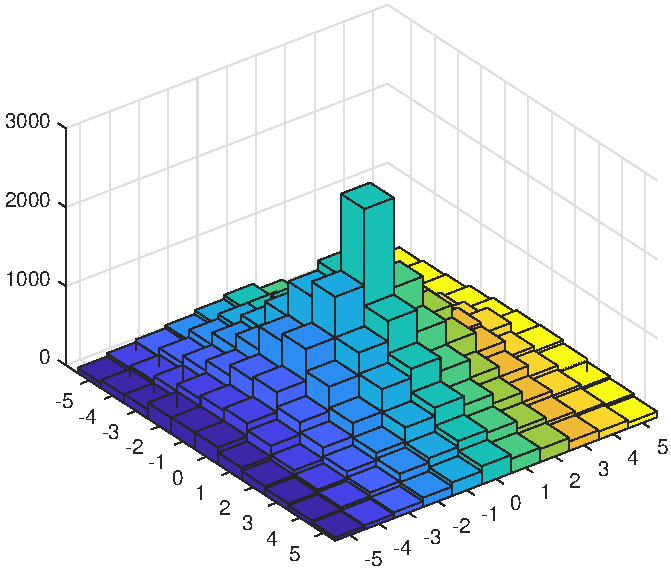
\includegraphics[width=1\textwidth]{./correlation_Lena.pdf}
\end{minipage}
}
\subfigure[Baboon]{
\begin{minipage}[t]{0.3\linewidth}
\centering
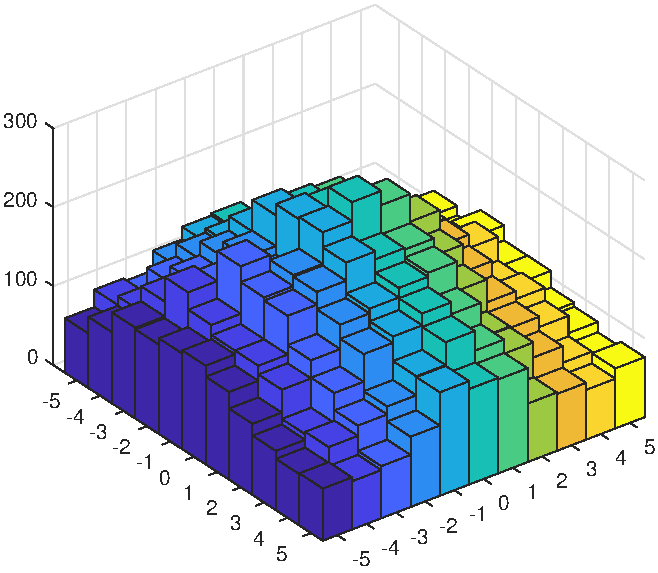
\includegraphics[width=1\textwidth]{./correlation_Baboon.pdf}
\end{minipage}
}
\subfigure[Airplane]{
\begin{minipage}[t]{0.3\linewidth}
\centering
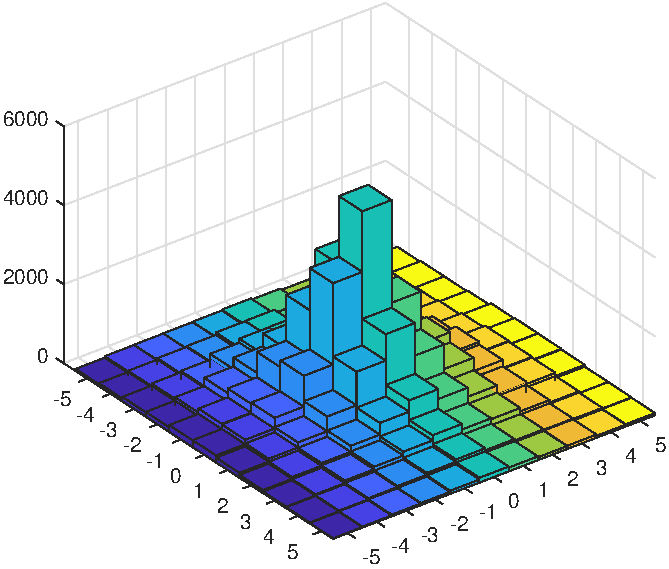
\includegraphics[width=1\textwidth]{./correlation_Airplane.pdf}
\end{minipage}
}			
\centering
\caption{Distribution of $(d_{\rm max},d_{\rm min})$, for three standard $512 \times 512$ sized gray-scale images Lena, Baboon and Airplane, with block size of $2 \times 2$.}
\label{fig:5}
\end{figure*}

First, inspired by previous works \cite{Li2013High(PVO),Peng2014Improved(PVO),Ou2014Reversible(PVO)}, we adopt the block selection strategy to select smooth blocks for histogram generation. More specifically, in order to evaluate the complexity of a block, the same as \cite{Ou2014Reversible(PVO)}, a block context is first defined as shown in Figure~\ref{fig:NL}, and then the complexity of a block is computed as the sum of the vertical and the horizontal absolute difference of every two adjacent pixels in the context. For a given threshold $T$, only the blocks with complexities less than $T$ are selected. The blocks with large complexities are considered as rough ones and will not be used in our data embedding. These blocks remain unchanged during the data embedding procedure. Then, the prediction-error pair $(d_{\rm max},d_{\rm min})$ is computed for each selected blocks, and the 2D histogram counting the distribution of $(d_{\rm max},d_{\rm min})$ is generated. After that, the data embedding will be conducted by modifying the generated 2D histogram.

\begin{figure}
\centering
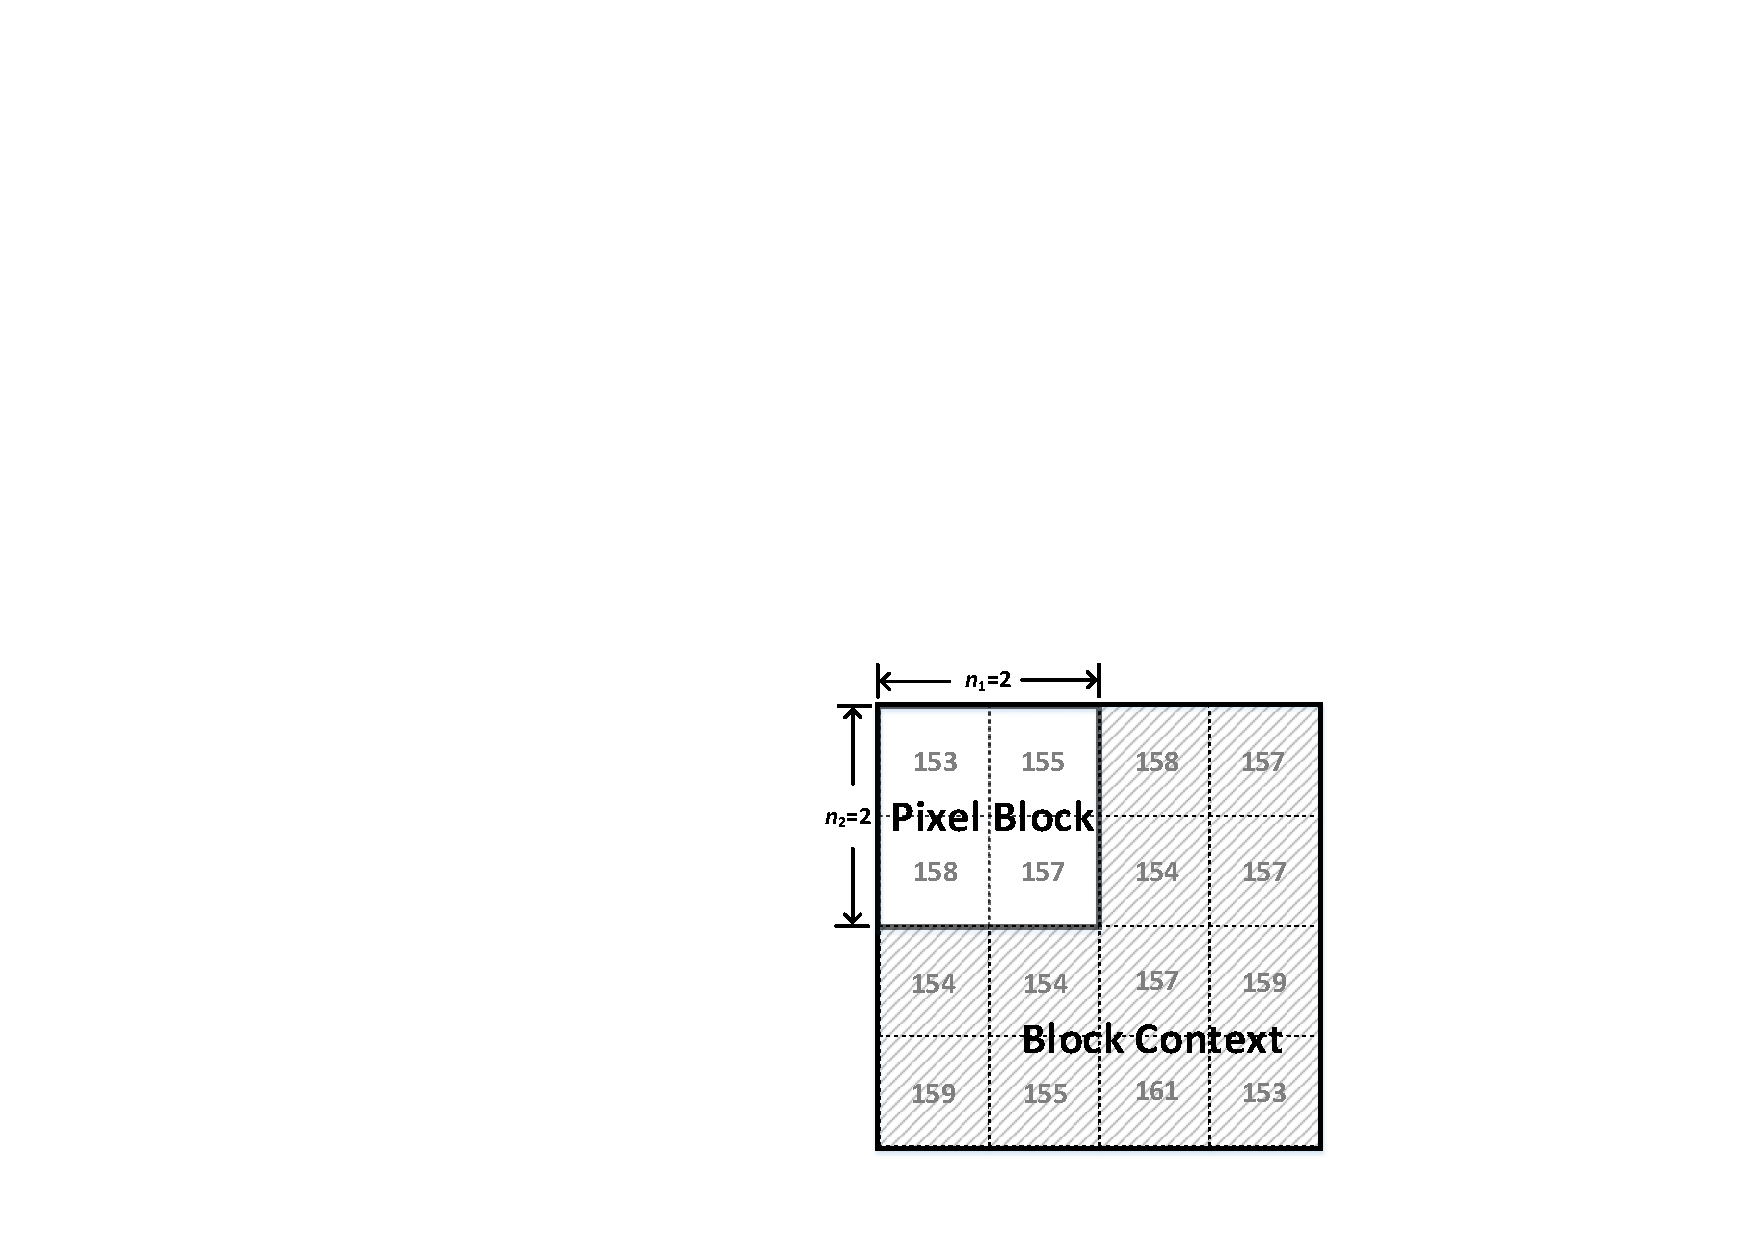
\includegraphics[width=0.25\textwidth]{./NL.pdf}
\caption{Context (shadow pixels) of a given block for complexity computation.}
\label{fig:NL}
\end{figure}

Clearly, one can directly apply the pairwise embedding mechanism of Ou \emph{et al.} \cite{Ou2013Pairwise(PEE)} to modify the generated histogram. For illustration, the pairwise embedding mechanism based on a 2D mapping is shown in Figure~\ref{fig:proposedCase}(a). The 2D mapping here is defined as a function
\begin{equation}\label{eq:function}
   f: \mathbb{Z}^2 \mapsto \mathcal{P}(\mathbb{Z}^2)
\end{equation}
where $\mathcal{P}(\mathbb{Z}^2)$ is the power set of $\mathbb{Z}^2$. For example, $f(0,0) = \{(0,0),(0,1),(1,0)\}$ means that in the data embedding process, the pair $(0,0)$ will be modified as one element of the set $\{(0,0),(0,1),(1,0)\}$ to embed $\log_23$ bits. Regard that, for a given embedding capacity, with pairwise embedding, the threshold $T$ is determined as the smallest one such that the embedding capacity can be satisfied with the generated histogram. For example, for the Baboon image with $2 \times 2$ sized blocks and an embedding capacity of 10,000 bits, the threshold $T$ is 235, and one can get a PSNR of 54.63 dB by applying the pairwise embedding to the corresponding histogram (this histogram is shown in Figure~\ref{fig:proposedCase}(c)). On the other hand, with the same block size     and complexity computation method, the PSNR of Peng \emph{et al.}'s method \cite{Peng2014Improved(PVO)} is just 54.34 dB. That is to say, compared with \cite{Peng2014Improved(PVO)}, 0.29 dB of improvement is obtained by using pairwise embedding. Obviously, the improvement is due to the utilization of the correlation between $d_{\rm max}$ and $d_{\rm min}$.

\begin{figure*}
\centering
\subfigure[]{
\begin{minipage}[t]{0.45\linewidth}
\centering
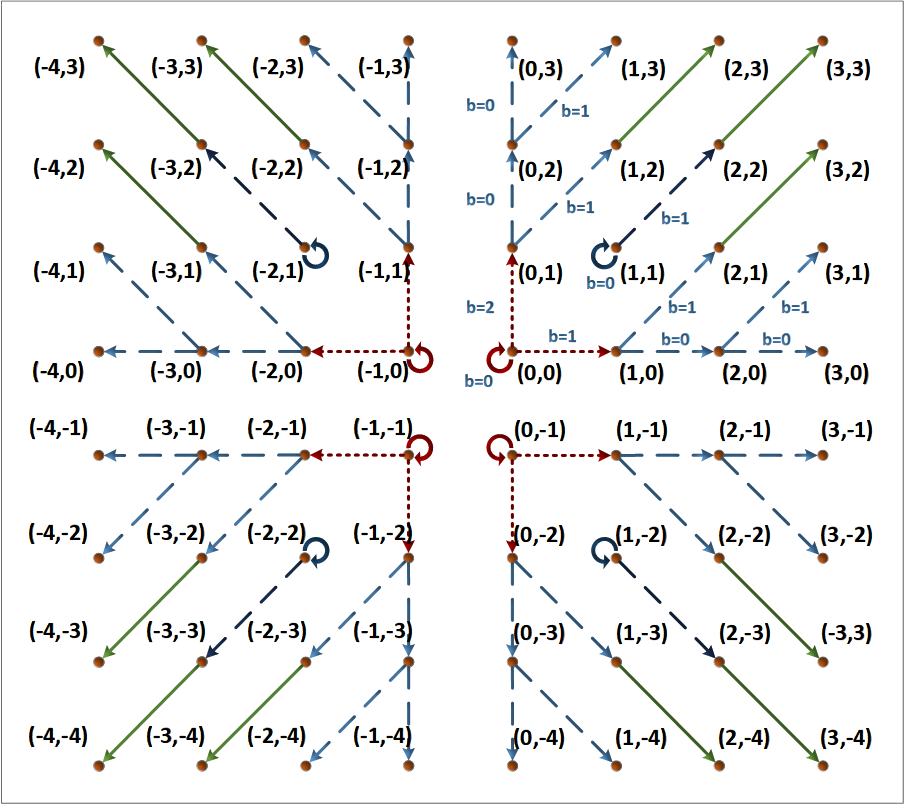
\includegraphics[width=1\textwidth]{./proposed.png}
\end{minipage}
}
\qquad\qquad
\subfigure[]{
\begin{minipage}[t]{0.45\linewidth}
\centering
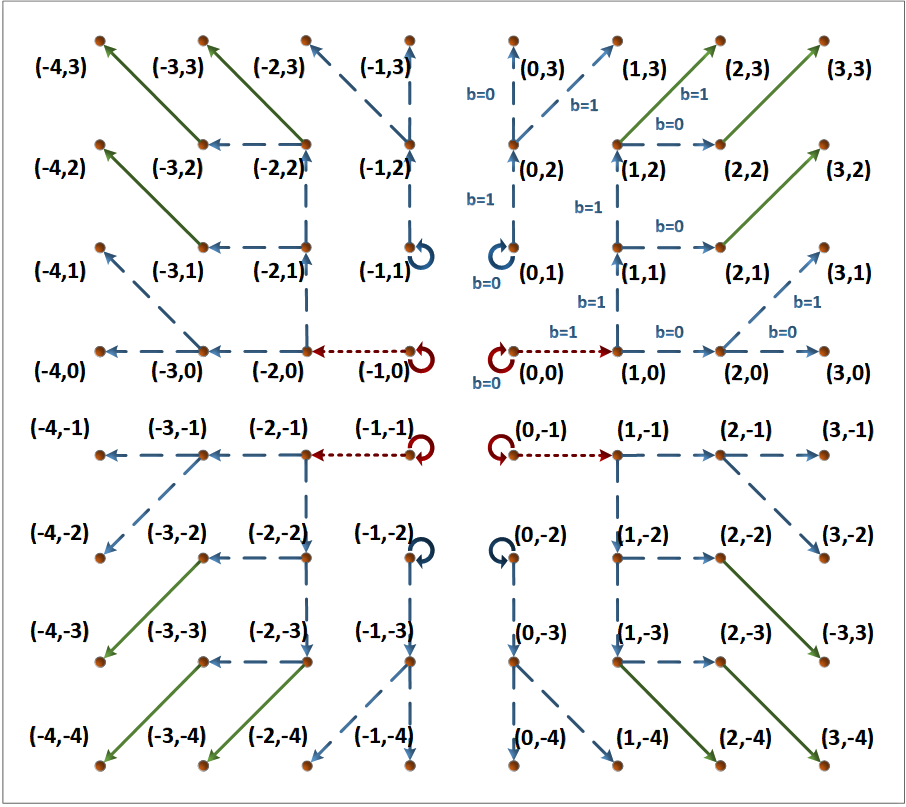
\includegraphics[width=1\textwidth]{./proposed2.png}
\end{minipage}
}

\subfigure[]{
\begin{minipage}[t]{0.35\linewidth}
\centering
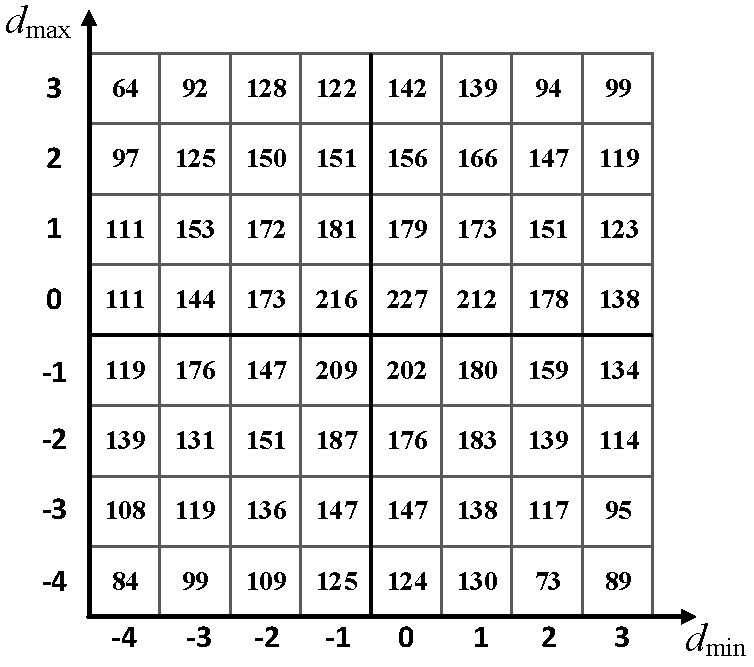
\includegraphics[width=1\textwidth]{./proposed_histogram.png}
\end{minipage}
}
\qquad\qquad
\subfigure[]{
\begin{minipage}[t]{0.35\linewidth}
\centering
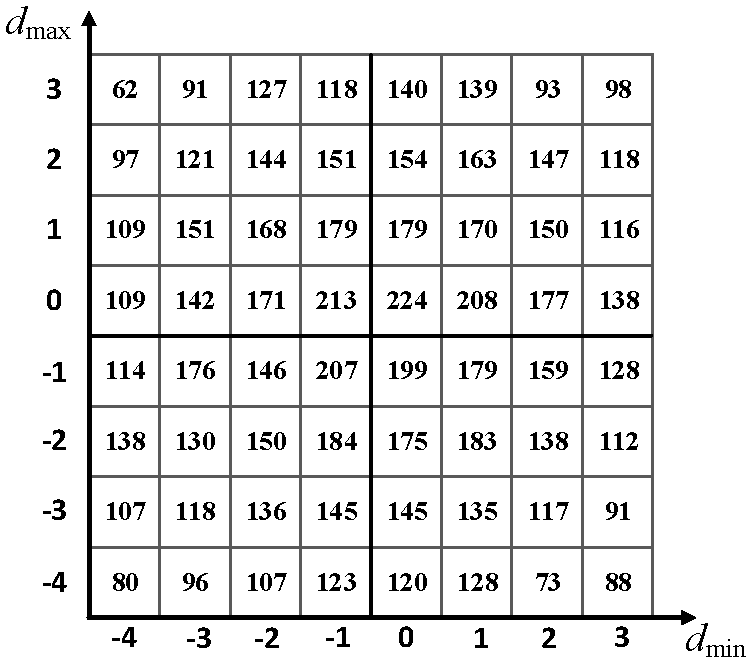
\includegraphics[width=1\textwidth]{./proposed_histogram2.png}
\end{minipage}
}
\centering
\caption{(a) 2D mapping of the pairwise embedding \cite{Ou2013Pairwise(PEE)},
         (b) Optimal 2D mapping obtained by the proposed method,
         (c) 2D histogram for the Baboon image with block size $2 \times 2$ and complexity threshold $T = 235$,
         (d) 2D histogram for the Baboon image with block size $2 \times 2$ and complexity threshold $T = 225$.}
\label{fig:proposedCase}
\end{figure*}

Based on pairwise embedding, the advantage of 2D histogram is verified. However, one can get better result since that, with the pairwise embedding mechanism of Ou \emph{et al.} \cite{Ou2013Pairwise(PEE)}, only a fixed modification manner is simply utilized for the 2D histogram. Actually, there are many ways for 2D histogram modification, and one can take the best one to optimize the embedding performance. Obviously, any 2D mapping defined in $\mathbb{Z}^2$ can derive a reversible embedding if it satisfies the following condition: for any $x \in \mathbb{Z}^2$, there exists unique $y \in \mathbb{Z}^2$ such that $x \in f(y)$. The detailed discussion on high dimensional mapping for RDH can be found in our previous work \cite{Li2016GeneralEx}. For clarity, the 2D mappings considered in the following context are the ones satisfying this condition. We then propose to use adaptive 2D mapping to enhance the performance.

We will exhaustively search all the 2D mappings and find the optimal one such that it can provide the required embedding capacity while the embedding distortion is minimized. Considering that the generated 2D histogram is usually symmetric for the four quadrants, we then suppose that the 2D mapping is symmetric as well. More specifically, we only consider the 2D mapping $f: \mathbb{Z}^2 \mapsto \mathcal{P}(\mathbb{Z}^2)$ which satisfies the following condition: for each $x \geq 0$ and $y \geq 0$, $f(x,y) = f(-x-1,y) = f(x,-y-1) = f(-x-1,-y-1)$. Moreover, as the generated 2D histogram is concentred on $(0,0)$, we only modify the pairwise embedding in a small local region $[0,K] \times [0,K]$ to derive the 2D mappings. That is to say, besides the region $[0,K] \times [0,K]$, each tested 2D mapping coincides with the mapping of pairwise embedding in the first quadrant. Here, to balance the embedding performance and the running time cost, the parameter $K$ is simply taken as 2. In this situation, we only need to test 1996 different 2D mappings in total. Then, for each 2D mapping, the same as the case of pairwise embedding, the complexity threshold $T$ is determined as the smallest one such that the embedding capacity can be satisfied with the generated 2D histogram. After managing all the 2D mappings, one can finally get the optimal mapping with minimized distortion. For example, for the Baboon image with $2 \times 2$ sized blocks and an embedding capacity of 10,000 bits, the optimal 2D mapping is shown in Figure~\ref{fig:proposedCase}(b), the corresponding complexity threshold $T = 225$, and the derived 2D histogram is shown in Figure~\ref{fig:proposedCase}(d). In this case, one can get a PSNR of 54.90 dB, and 0.27 dB of improvement is obtained compared with pairwise embedding. We see then, with optimal 2D mapping, the method \cite{Peng2014Improved(PVO)} is further improved.

Similar with the previous methods \cite{Li2013High(PVO),Peng2014Improved(PVO)}, the above embedding procedure is implemented several times for different  block size $n_1,n_2 \in \{2,3,4,5\}$, and the best embedding result is taken as our final embedding result.

\textcolor[rgb]{1.00,0.00,0.00}{
Finally, before closing this section, we describe how to overcome the overflow/underflow problem. As many previous RDH works, a location map denoted $LM$ is used in the proposed method to record all the locations of pixels with value 0 or 255. Particularly, we set $LM(i) = 1$ if the $i$-th pixel value is 0 or 255, otherwise, we take $LM(i) = 0$. Meanwhile, before data embedding, all pixels with value 0 are modified to 1, and all pixels with value 255 are modified to 254. Then, the lossless compressed location map will be embedded into the cover image as a part of the auxiliary information for blind extraction. Specifically, in the proposed method, the auxiliary information has a total of $25 + 2\left \lceil \log_2N \right \rceil + l_{\rm CLM}$ bits including
\begin{itemize}
  \item block size parameters $n_1$ and $n_2$ (4 bits),
  \item block complexity threshold $T$ (10 bits),
  \item end position for recording the last data embedding position ($\left \lceil \log_2N \right \rceil$ bits),
  \item length of the compressed location map ($\left \lceil \log_2N \right \rceil$ bits),
  \item index of the optimal 2D mapping (11 bits),
  \item the lossless compressed location map ($l_{\rm CLM}$ bits).
\end{itemize}
Here, $N$ is the number of cover pixels.
}

\section{Experimental results} \label{Experimental Results}

In this section, the proposed method is evaluated by comparing it with the original PVO-based method \cite{Li2013High(PVO)}, the improved PVO-based method \cite{Peng2014Improved(PVO)}, and a recently proposed PVO-based method \cite{Ou2014Reversible(PVO)}. Eight standard $512\times 512$ sized gray-scale bitmap images including Lena, Baboon, Airplane, Barbara, Lake, Boat, Peppers and Elaine, are used in the experiment for evaluation.
\textcolor[rgb]{1.00,0.00,0.00}{
The proposed method is implemented by using C++ on Visual Studio 2017 with a personal laptop (ThinkPad X280). It costs less than 0.01s to generate all 1996 2D mappings. Moreover, the embedding process can be completed within five seconds for a given embedding capacity (see Table \ref{tab:3}) and it requires $8.65$ MB of memory to store all 2D mappings.
}

\begin{table*}
\scriptsize
\centering
\caption{Time cost (in seconds) of the proposed method with different embedding capacities.}
\setlength{\tabcolsep}{4.3mm}{
\begin{tabular}{ccccccccccccc}
\hline
{       }    & Lena  & Baboon  & Airplane  & Barbara  & Lake  & Boat  & Peppers  & Elaine & Average   \\
\hline
{5,000  bits }   & 2.03  & 3.92    & 2.11      & 2.30     & 2.65  & 2.58  & 2.34     & 2.66   & 2.57    \\
\hline
{10,000 bits}   & 2.98  & 4.63    & 2.89      & 3.61     & 3.75  & 3.71  & 3.44     & 3.88   & 3.61    \\
\hline
{15,000 bits}   & 3.76  &  --     & 3.65      & 4.11     & 4.33  & 4.34  & 4.17     & 4.50   & 4.09    \\
\hline
{20,000 bits}   & 4.30  &  --     & 4.18      & 4.33     & 4.39  & 4.63  & 4.60     & 4.78   & 4.45    \\
\hline
{25,000 bits}   & 4.53  &  --     & 4.39      & 4.35     & 4.57  & 4.54  & 4.74     & --     & 4.52    \\
\hline
{30,000 bits}   & 4.70  &  --     & 4.65      & 4.53     & --    & --    & 4.97     & --     & 4.71    \\
%\hline
%{3,5000 bits}   & 4.76  &  --     & 4.57      & --       & --    & --    & --       & --     & 4.67    \\
%\hline
%{4,0000 bits}   & --    &  --     & 4.70      & --       & --    & --    & --       & --     & 4.70    \\
%\hline
%{4,5000 bits}   & --    &  --     & 4.63      & --       & --    & --    & --       & --     & 4.63    \\
\hline
\end{tabular}
}
\label{tab:3}
\end{table*}

First, for a given embedding capacity of 10,000 bits and 20,000 bits, we show the optimal parameters (including the block size $(n_1,n_2)$ and the complexity threshold $T$) of the proposed method in Table~\ref{tab:10000bitsOfMethods} and Table~\ref{tab:20000bitsOfMethods}. The parameters are rather different for different images. We may then conclude that it is necessary to test different block size for PVO-based methods, and it is reasonable to take large sized blocks for low embedding capacity. Moreover, for a better illustration, the optimal 2D mappings for some test images with different embedding capacities, are shown in Figure~\ref{fig:experimentMapping}, and the adaptivity can be observed from this figure. For brevity, only the 2D mapping in the first quadrant is plotted in Figure~\ref{fig:experimentMapping}. Figure~\ref{fig:capacity} shows the embedding performance presented by the capacity-distortion curves. It can be seen that the proposed method is superior to the compared methods with a higher PSNR whatever the cover image or the embedding capacity is.

\begin{table*}
\scriptsize
\centering
\caption{Comparison of PSNR (dB) among the proposed method and the PVO-based methods of Li \emph{et al.} \cite{Li2013High(PVO)}, Peng \emph{et al.} \cite{Peng2014Improved(PVO)}, Ou \emph{et al.} \cite{Ou2014Reversible(PVO)}. The embedding capacity is 10,000 bits. The optimal parameters of the proposed method and the compared methods are also listed.}
\setlength{\tabcolsep}{3mm}{
\begin{tabular}{lcclcclcclccl}
\toprule
\multirow{2}{*}{Images} & \multicolumn{3}{c}{Li \emph{et al.}} & \multicolumn{3}{c}{Peng \emph{et al.}} & \multicolumn{3}{c}{Ou \emph{et al.}} & \multicolumn{3}{c}{Proposed}\\
\cmidrule(r){2-4} \cmidrule(r){5-7} \cmidrule(r){8-10} \cmidrule(r){11-13}
&  PSNR      &  $(n_1, n_2)$   &   $T$
&  PSNR      &  $(n_1, n_2)$   &   $T$
&  PSNR      &  $(n_1, n_2)$   &   $(T_1, T_2)$
&  PSNR      &  $(n_1, n_2)$   &   $T$ \\
\midrule
%\hline
%{Images}                & Li \emph{et al.}   & Peng \emph{et al.}    & Ou \emph{et al.}  & Proposed\\
%\hline
Lena                    & 60.34  & (5,2) & 9    & 60.49  & (4,3) & 9    & 60.59  & (4,2) & (69,40)      & \textbf{61.09}  & (4,2) & 67  \\ % 0.01
Baboon                  & 53.46  & (2,2) & 12   & 53.58  & (3,2) & 61   & 54.48  & (2,2) & (238,132)    & \textbf{54.90}  & (2,2) & 225 \\ % 0.01
Airplane                & 62.10  & (2,4) & 5    & 62.97  & (5,2) & 4    & 63.29  & (2,2) & (21,2)       & \textbf{63.87}  & (3,2) & 24  \\ % 0.01
Barbara                 & 60.39  & (4,2) & 8    & 60.48  & (3,3) & 7    & 60.59  & (3,2) & (57,16)      & \textbf{61.04}  & (2,3) & 54  \\ % 0.01
Lake                    & 58.15  & (4,2) & 14   & 58.81  & (2,4) & 10   & 59.36  & (2,2) & (66,31)      & \textbf{59.74}  & (2,2) & 61  \\ % 0.03
Boat                    & 58.05  & (2,4) & 13   & 58.26  & (2,5) & 16   & 58.23  & (2,4) & (146,74)     & \textbf{58.66}  & (2,4) & 140 \\ % 0.01
Peppers                 & 58.87  & (3,3) & 10   & 58.97  & (3,4) & 13   & 59.18  & (3,3) & (107,73)     & \textbf{59.63}  & (3,3) & 107 \\ % 0.01
Elaine                  & 56.84  & (3,3) & 19   & 57.37  & (4,3) & 23   & 57.37  & (3,2) & (131,74)     & \textbf{58.07}  & (2,2) & 81  \\ % 0.02
\hline
Average                 & 58.52  &       &      & 58.86  &       &      & 59.13  &       &              & \textbf{59.63}  &       &     \\
\hline
\end{tabular}
}
\label{tab:10000bitsOfMethods}
\end{table*}


\begin{table*}
\scriptsize
\centering
\caption{Comparison of PSNR (dB) among the proposed method and the PVO-based methods of Li \emph{et al.} \cite{Li2013High(PVO)}, Peng \emph{et al.} \cite{Peng2014Improved(PVO)}, Ou \emph{et al.} \cite{Ou2014Reversible(PVO)}. The embedding capacity is 20,000 bits. The optimal parameters of the proposed method and the compared methods are also listed.}
\setlength{\tabcolsep}{3mm}{
\begin{tabular}{lcclcclcclccl}
\toprule
\multirow{2}{*}{Images} & \multicolumn{3}{c}{Li \emph{et al.}} & \multicolumn{3}{c}{Peng \emph{et al.}} & \multicolumn{3}{c}{Ou \emph{et al.}} & \multicolumn{3}{c}{Proposed}\\
\cmidrule(r){2-4} \cmidrule(r){5-7} \cmidrule(r){8-10} \cmidrule(r){11-13}
&  PSNR      &  $(n_1, n_2)$   &   $T$
&  PSNR      &  $(n_1, n_2)$   &   $T$
&  PSNR      &  $(n_1, n_2)$   &   $(T_1, T_2)$
&  PSNR      &  $(n_1, n_2)$   &   $T$ \\
\midrule
Lena                    & 56.20  & (3,2) & 9    & 56.56  & (4,2) & 12   & 56.58  & (3,2) & (83,53)      & \textbf{57.19}  & (3,2) & 86  \\ % 0.01
Airplane                & 58.20  & (2,3) & 6    & 59.07  & (2,4) & 5    & 59.33  & (2,2) & (30,15)      & \textbf{59.98}  & (2,2) & 25  \\ % 0.01
Barbara                 & 55.43  & (2,2) & 4    & 56.20  & (3,2) & 11   & 56.50  & (2,2) & (69,27)      & \textbf{57.17}  & (2,2) & 59  \\ % 0.01
Lake                    & 53.39  & (2,2) & 8    & 53.53  & (2,2) & 6    & 54.29  & (2,2) & (133,67)     & \textbf{54.62}  & (2,2) & 123 \\ % 0.03
Boat                    & 53.29  & (2,2) & 9    & 53.83  & (2,3) & 33   & 53.76  & (2,2) & (134,52)     & \textbf{54.19}  & (2,2) & 123 \\ % 0.01
Peppers                 & 54.66  & (3,2) & 22   & 54.77  & (3,2) & 10   & 54.93  & (3,2) & (133,95)     & \textbf{55.40}  & (3,2) & 143 \\ % 0.01
Elaine                  & 52.36  & (2,2) & 12   & 52.65  & (2,2) & 7    & 52.71  & (2,2) & (170,65)     & \textbf{53.27}  & (2,2) & 144 \\ % 0.02
\hline
Average                 & 54.79  &       &      & 55.23  &       &      & 55.44  &       &              & \textbf{55.97}  &       &     \\
\hline
\end{tabular}
}
\label{tab:20000bitsOfMethods}
\end{table*}

%\begin{table}
%\centering
%\caption{Optimal parameters of the proposed method for the embedding capacity of 10,000 bits.}
%\setlength{\tabcolsep}{5mm}
%\setlength{\abovecaptionskip}{0pt}
%\setlength{\belowcaptionskip}{20pt}
%\begin{tabular}{lcccl}
%\hline
%{Images}    & PSNR(dB)     & $n_1$      & $n_2$     & $T$    \\
%\hline
%Lena        & 61.09        & 4          & 2         & 67     \\
%Baboon      & 54.90        & 2          & 2         & 225    \\
%Airplane    & 63.87        & 3          & 2         & 24     \\
%Barbara     & 61.04        & 2          & 3         & 54     \\
%Lake        & 59.74        & 2          & 2         & 61     \\
%Boat        & 58.66        & 2          & 4         & 140    \\
%Peppers     & 59.63        & 3          & 3         & 107    \\
%Elaine      & 58.07        & 2          & 2         & 81     \\
%\hline
%\end{tabular}
%\label{tab:10000bitsOfImgs}
%\end{table}

\begin{figure*}
\centering
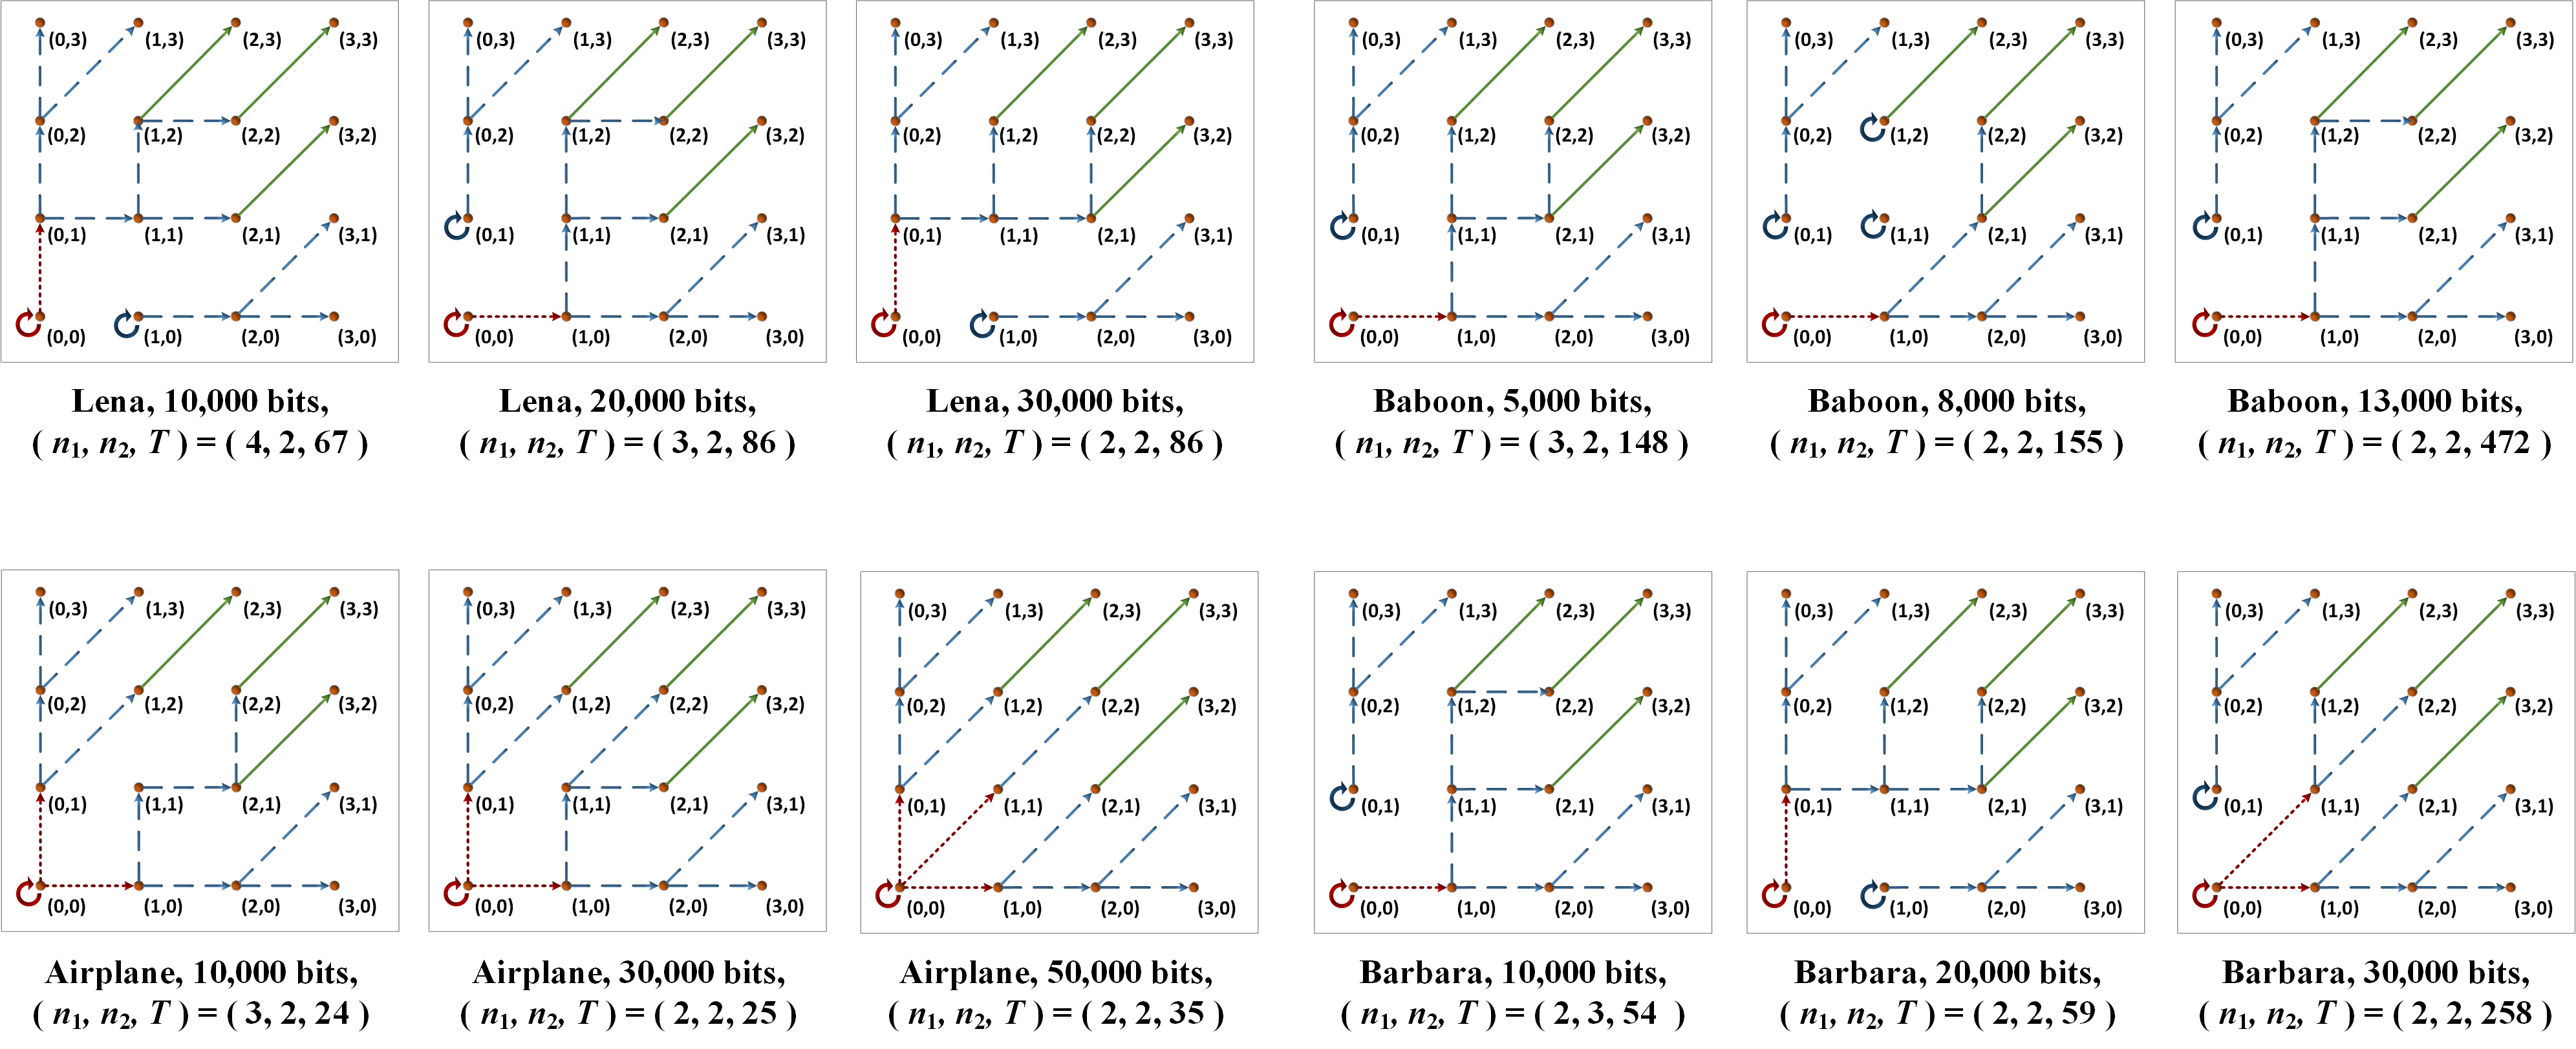
\includegraphics[width=1\textwidth]{./experiment_mapping.png}
\centering
\caption{Optimal 2D mappings for some test images with different embedding capacities.}
\label{fig:experimentMapping}
\end{figure*}

%\begin{table}
%\centering
%\caption{Optimal parameters of the proposed method for the embedding capacity of 20,000 bits.}
%\setlength{\tabcolsep}{5mm}
%\setlength{\abovecaptionskip}{0pt}
%\setlength{\belowcaptionskip}{20pt}
%\begin{tabular}{lcccl}
%\hline
%{Images}    & PSNR(dB)     & $n_1$      & $n_2$     & $T$      \\
%\hline
%Lena        & 57.19        & 3          & 2         & 86     \\
%Airplane    & 59.98        & 2          & 2         & 25     \\
%Barbara     & 57.17        & 2          & 2         & 59     \\
%Lake        & 54.62        & 2          & 2         & 123     \\
%Boat        & 54.19        & 2          & 2         & 123    \\
%Peppers     & 55.40        & 3          & 2         & 143    \\
%Elaine      & 53.27        & 2          & 2         & 144     \\
%\hline
%\end{tabular}
%\label{tab:20000bitsOfImgs}
%\end{table}

\begin{figure*}
\centering
\subfigure{
\begin{minipage}[t]{0.42\linewidth}
\centering
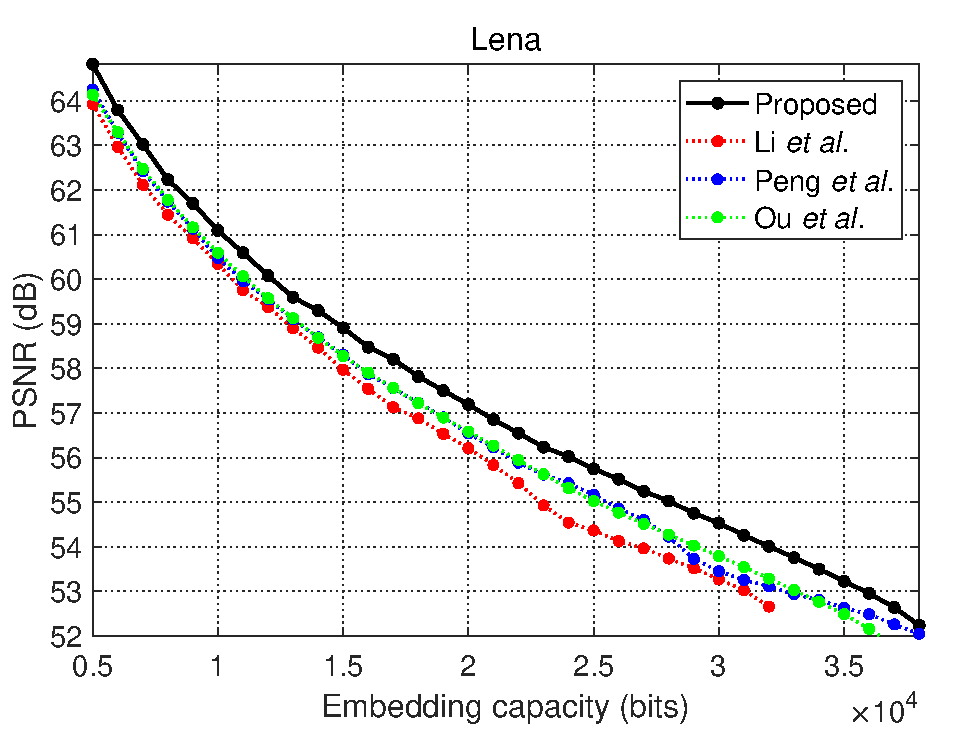
\includegraphics[width=1\textwidth]{./Lena.pdf}
\end{minipage}
}
\subfigure{
\begin{minipage}[t]{0.42\linewidth}
\centering
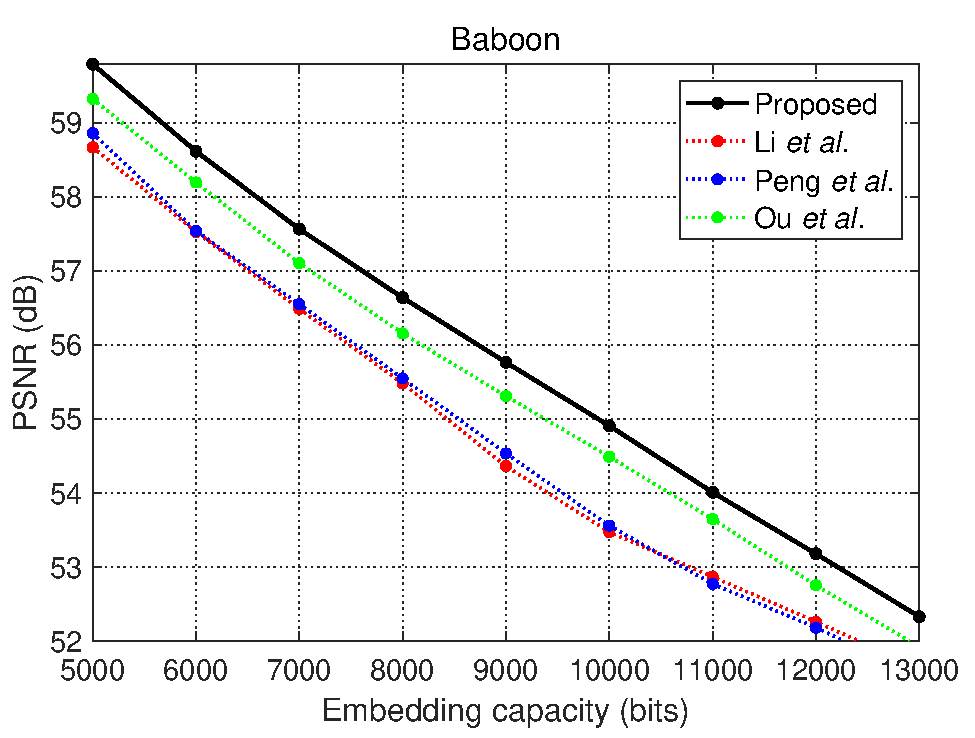
\includegraphics[width=1\textwidth]{./Baboon.pdf}
\end{minipage}
}

\subfigure{
\begin{minipage}[t]{0.42\linewidth}
\centering
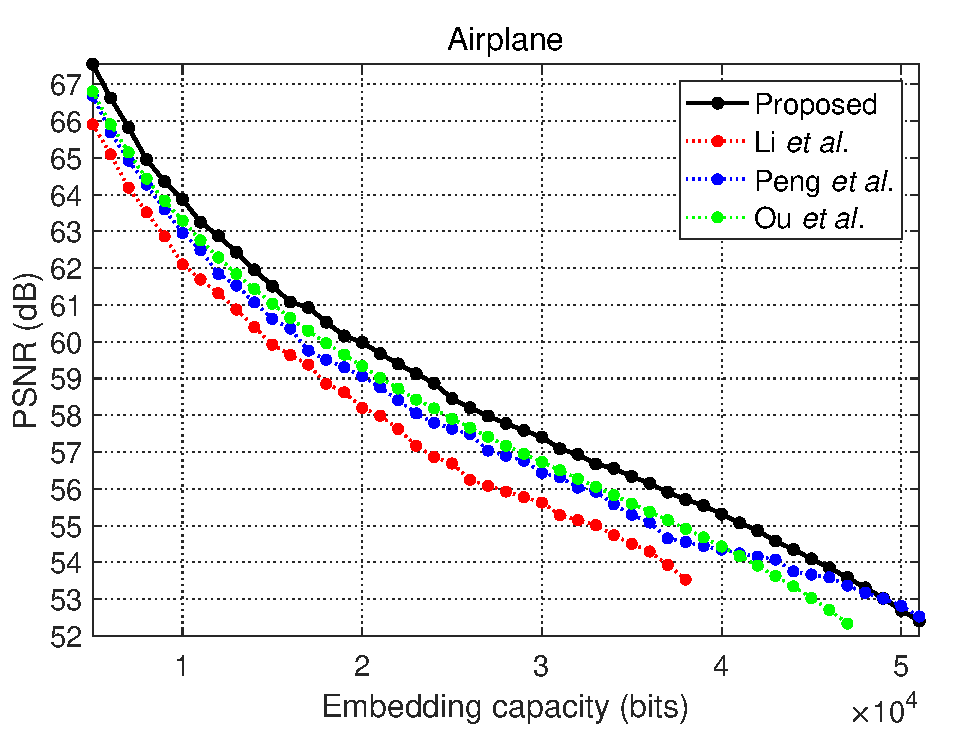
\includegraphics[width=1\textwidth]{./Airplane.pdf}
\end{minipage}
}
\subfigure{
\begin{minipage}[t]{0.42\linewidth}
\centering
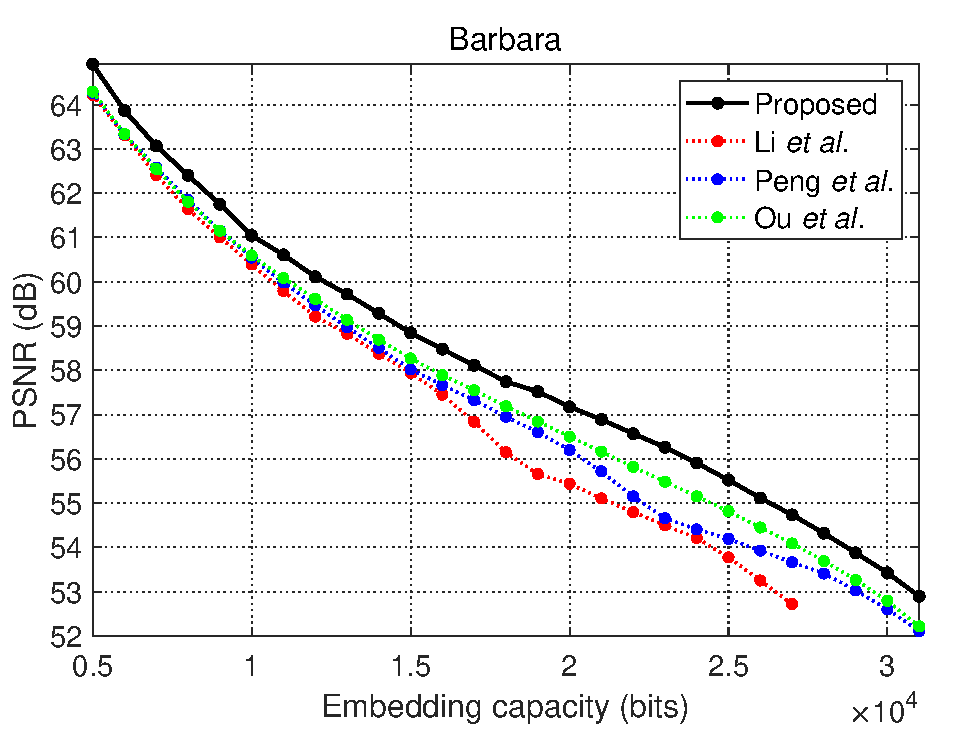
\includegraphics[width=1\textwidth]{./Barbara.pdf}
\end{minipage}
}

\subfigure{
\begin{minipage}[t]{0.42\linewidth}
\centering
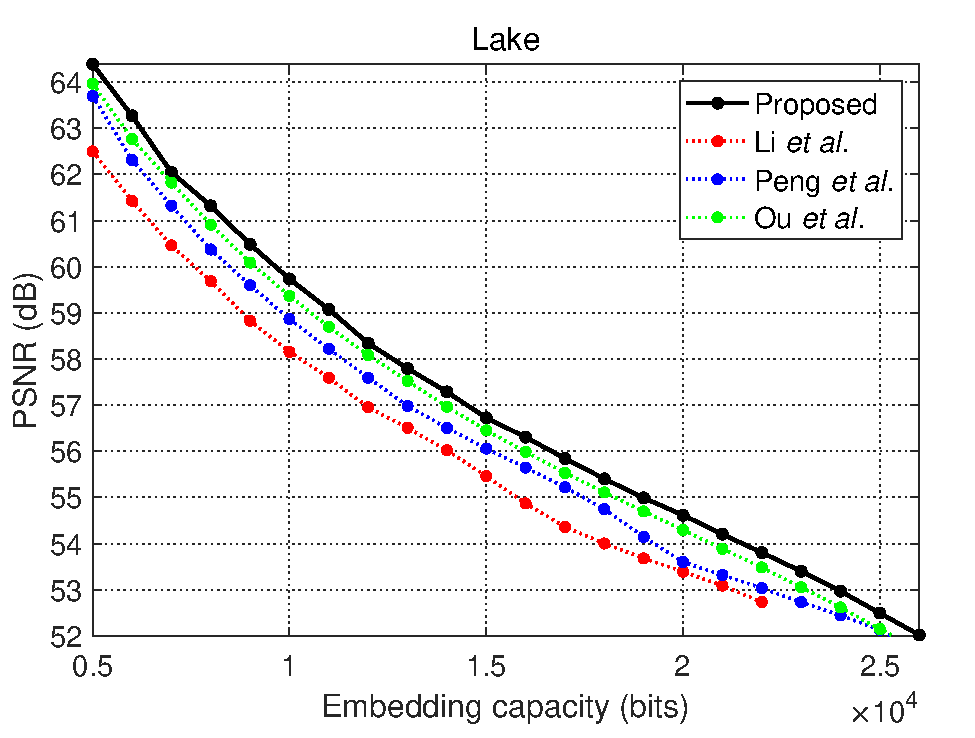
\includegraphics[width=1\textwidth]{./Lake.pdf}
\end{minipage}
}
\subfigure{
\begin{minipage}[t]{0.42\linewidth}
\centering
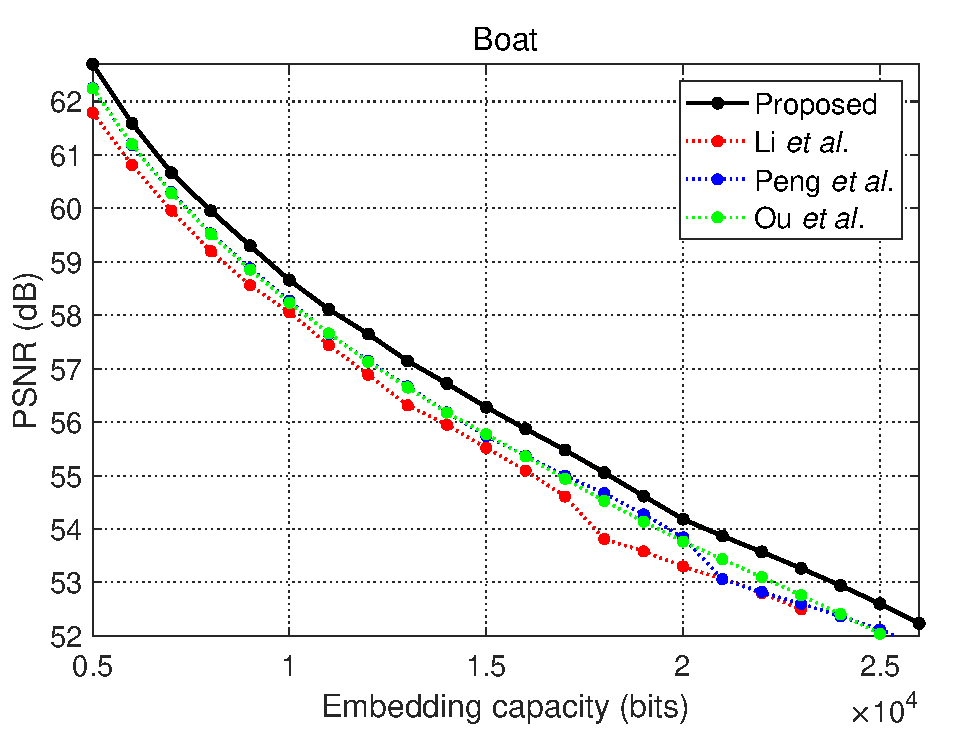
\includegraphics[width=1\textwidth]{./Boat.pdf}
\end{minipage}
}

\subfigure{
\begin{minipage}[t]{0.42\linewidth}
\centering
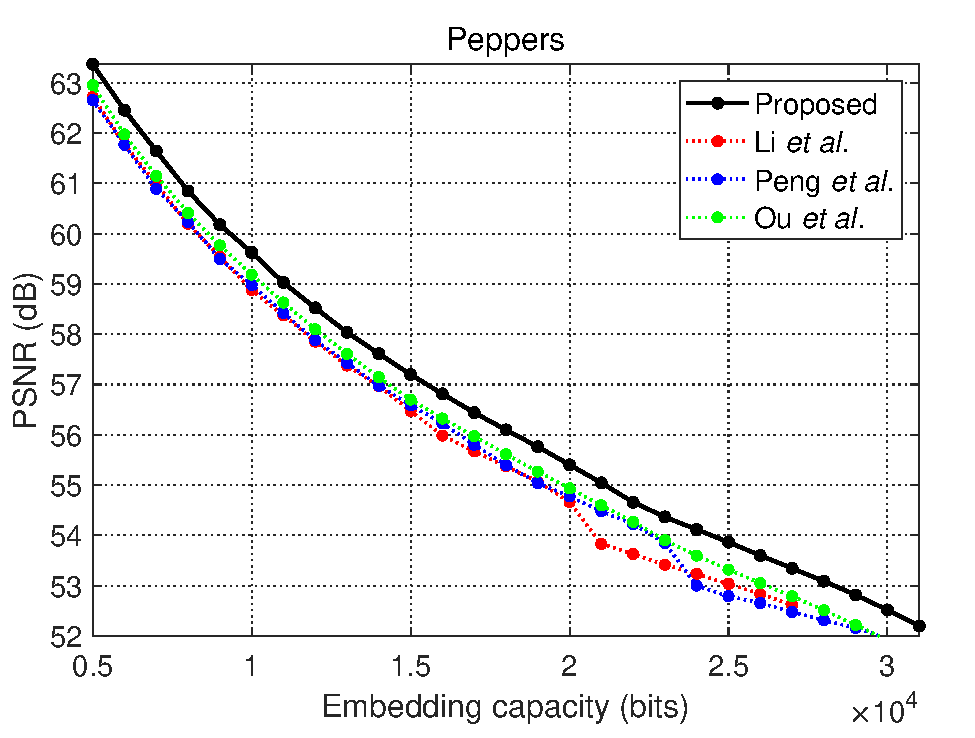
\includegraphics[width=1\textwidth]{./Peppers.pdf}
\end{minipage}
}
\subfigure{
\begin{minipage}[t]{0.42\linewidth}
\centering
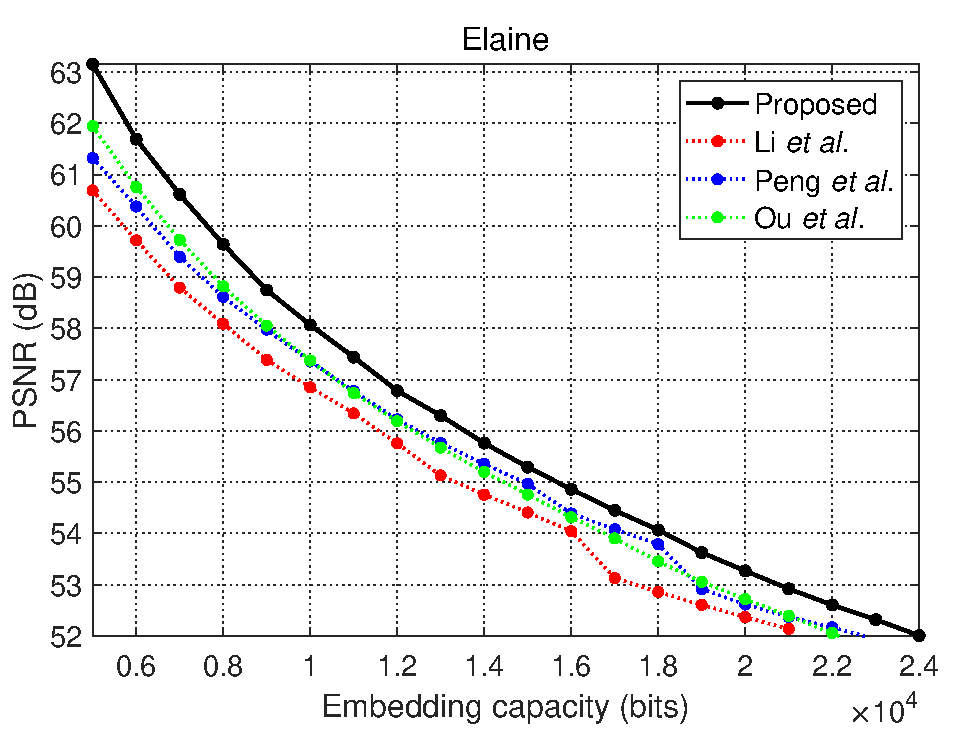
\includegraphics[width=1\textwidth]{./Elaine.pdf}
\end{minipage}
}

\centering
\caption{Performance comparison between the proposed method and Li \emph{et al.}'s method \cite{Li2013High(PVO)}, Peng \emph{et al.}'s  method \cite{Peng2014Improved(PVO)}, and Ou \emph{et al.}'s method \cite{Ou2014Reversible(PVO)}.}
\label{fig:capacity}       % Give a unique label
\end{figure*}

For the original PVO-based method \cite{Li2013High(PVO)}, as we have mentioned, the smooth blocks are not exploited for data embedding. As a result, this method is less efficient compared with the other tested methods. According to Table~\ref{tab:10000bitsOfMethods} and Table~\ref{tab:20000bitsOfMethods}, for a given embedding capacity of 10,000 and 20,000 bits, compared with \cite{Li2013High(PVO)}, our method can get better embedding result with an increase of PSNR of 1.11 dB and 1.18 dB in average, respectively. Peng \emph{et al.}'s method \cite{Peng2014Improved(PVO)} is an improvement of \cite{Li2013High(PVO)}. Although efficient, its embedding performance is still unsatisfactory with independent modification for $d_{\rm max}$ and $d_{\rm min}$. According to Table~\ref{tab:10000bitsOfMethods} and Table~\ref{tab:20000bitsOfMethods}, compared with this method, our method can respectively get an increase of PSNR
of 0.77 dB and 0.74 dB in average, for an embedding capacity of 10,000 and 20,000 bits. The advantage of the proposed method mainly lies in the utilization of 2D histogram and its adaptive modification. Notice that, in Table~\ref{tab:10000bitsOfMethods} and Table~\ref{tab:20000bitsOfMethods}, the embedding parameters which provides the best embedding results for the comparison methods are also listed in these two tables.

The so-called PVO-$k$ method \cite{Ou2014Reversible(PVO)} is another improvement of \cite{Li2013High(PVO)}. For this method, if more than one pixel
taking the largest value in a given block, all these pixels will be simultaneously modified in a same way for data embedding. This method is verified better than \cite{Li2013High(PVO)}, however, the smooth blocks are still not utilized for data embedding (e.g., the block whose pixel values are identical). According to Table~\ref{tab:10000bitsOfMethods} and Table~\ref{tab:20000bitsOfMethods}, for an embedding capacity of 10,000 and 20,000 bits, compared with \cite{Ou2014Reversible(PVO)}, our method can get better embedding result with an increase of PSNR of 0.50 dB and 0.53 dB in average, respectively.

\section{Conclusion} \label{Conclusion}

Based on PVO and adaptive pairwise modification, an improved RDH method is proposed in this paper. After dividing the cover image into non-overlapping equal-sized blocks, unlike previous PVO-based works \cite{Li2013High(PVO),Peng2014Improved(PVO),Ou2014Reversible(PVO)}, the prediction-errors for the largest and smallest pixel values of each block are jointed as a pair. Then, the secret data is embedded into the cover image by adaptively modifying the 2D histogram which is generated based on the prediction-error pairs of smooth image blocks. The proposed method is experimentally verified better than the previous works \cite{Li2013High(PVO),Peng2014Improved(PVO),Ou2014Reversible(PVO)}. To enhance the embedding capacity and further improve the embedding performance, one possible direction of PVO-based RDH approach is to take more pixels in each block for data embedding.


\begin{thebibliography}{28}

\bibitem{Cox2007Digital}
Cox, I., Miller, M., Bloom, J., Fridrich, J., and Kalker, T., Digital Watermarking and Steganography.
San Mateo, CA, USA: Morgan Kaufmann,2007.

\bibitem{Fridrich2009Steganography}
Fridrich, J., Steganography in Digital Media: Principles, Algorithms, and Applications.
Cambridge, U.K.: Cambridge Univ. Press, 2009.

\bibitem{Zhang2006Efficient}
Zhang, X., Wang, S.: Efficient Steganographic Embedding by Exploiting Modification Direction.
IEEE Commun. Lett.  \textbf{10}(11),  781--783 (2006)

\bibitem{Zhang2011Reference}
Zhang, X., Wang, S., Qian, Z., Feng, G.: Reference Sharing Mechanism for Watermark Self-Embedding.
IEEE Trans. Image Process.  \textbf{20}(2),  485--495 (2011)

\bibitem{Qin2014Novel}
Qin, C., Chang, C.C., Chiu, Y.P.: A Novel Joint Data-Hiding and Compression Scheme Based on SMVQ and Image Inpainting.
IEEE Trans. Image Process.  \textbf{23}(3),  969--978 (2014)

\bibitem{Qin2015Effective}
Qin, C., Zhang, X.: Effective reversible data hiding in encrypted image with privacy protection for image content.
J. Vis. Commun. Image R.  \textbf{31},  154--164 (2015)

\bibitem{Hong2017Coherent}
Hong, R., Li, L., Cai, J., Tao, D., Wang, M., Tian, Q.: Coherent Semantic-Visual Indexing for Large-Scale Image Retrieval in the Cloud.
IEEE Trans. Image Process.  \textbf{26}(9),  412    8--4138 (2017)

\bibitem{Ma2019Selection}
Ma, Y., Luo, X., Li, X., Bao, Z., Zhang, Y.: Selection of Rich Model Steganalysis Features Based on Decision Rough Set $\alpha$-Positive Region Reduction.
IEEE Trans. Circuits Syst. Video Technol.  \textbf{29}(12),  336--350 (2019)

\bibitem{Tian2003Reversible(DE)}
Tian, J.: Reversible data embedding using a difference expansion.
IEEE Trans. Circuits Syst. Video Technol.  \textbf{13}(8),  890--896 (2003)

\bibitem{Ni2006Reversible(HS)}
Ni, Z., Shi, Y.Q., Ansari, N., Su, W.: Reversible data hiding.
IEEE Trans. Circuits Syst. Video Technol.  \textbf{16}(3),  354--362 (2006)

\bibitem{Thodi2007Expansion(PEE)}
Thodi, D.M., Rodriguez, J.J.: Expansion embedding techniques for reversible watermarking.
IEEE Trans. Image Process.  \textbf{16}(3),  721--730 (2007)

\bibitem{Hong2009Reversible(PEE)}
Hong, W., Chen, T.S., Shiu, C.W.: Reversible data hiding for high quality images using modification of prediction errors.
J. Syst. Softw.  \textbf{82}(11),  1833-1842 (2009)

\bibitem{Sachnev2009Reversible(PEE)}
Sachnev, V., Kim, H.J., Nam, J., Suresh, S., Shi, Y.Q.: Reversible watermarking algorithm using sorting and prediction.
IEEE Trans. Circuits Syst. Video Technol.  \textbf{19}(7),  989--999 (2009)

\bibitem{coatrieux2009reversible(adaptive)}
Coatrieux, G., Le~Guillou, C., Cauvin, J.M., Roux, C.: Reversible watermarking for knowledge digest embedding and reliability control in medical images.
IEEE Trans. Inf. Technol. Biomed.  \textbf{13}(2),  158--165 (2009)

\bibitem{Li2011Efficient(PEE)}
Li, X., Yang, B., Zeng, T.: Efficient reversible watermarking based on adaptive prediction-error expansion and pixel selection.
IEEE Trans. Image Process. \textbf{20}(12),  3524--3533 (2011)

\bibitem{Coltuc2011Improved(PEE)}
Coltuc, D.: Improved embedding for prediction-based reversible watermarking.
IEEE Trans. Inf. Forens. Secur.  \textbf{6}(3),  873--882 (2011)

\bibitem{Hong2011Adaptive(PEE)}
Hong, W.: Adaptive reversible data hiding method based on error energy control and histogram shifting.
Optics Communications.  \textbf{285}(2),  101--108 (2011)

\bibitem{Ou2013Pairwise(PEE)}
Ou, B., Li, X., Zhao, Y., Ni, R., Shi, Y.Q.: Pairwise prediction-error expansion for efficient reversible data hiding.
IEEE Trans. Image Process.  \textbf{22}(12),  5010--5021 (2013)

\bibitem{Li2013A(DE)}
Li, X., Zhang, W., Gui, X., Yang, B.: A novel reversible data hiding scheme based on two-dimensional difference-histogram modification.
IEEE Trans. Inf. Forens. Secur.  \textbf{8}(7),  1091--1100 (2013)

\bibitem{Qin2013An(PEE)}
Qin, C., Chang, C.C., Huang, Y.H., Liao, L.T.: An inpainting-assisted reversible steganographic scheme using a histogram shifting mechanism.
IEEE Trans. Circuits Syst. Video Technol.  \textbf{23}(7),  1109--1118 (2013)

\bibitem{Li2013General(HS)}
Li, X., Li, B., Yang, B., Zeng, T.: General framework to histogram-shifting-based reversible data hiding.
IEEE Trans. Image Process.  \textbf{22}(6),  2181--2191 (2013)

\bibitem{xuan2013optimal(adaptive)}
Xuan, G., Tong, X., Teng, J., Zhang, X., Shi, Y.Q.: Optimal histogram-pair and prediction-error based image reversible data hiding.
in Proc. IWDW, pp. 368--383. Springer(2013)

\bibitem{dragoi2014local}
Dragoi, I.C., Coltuc, D.: Local-prediction-based difference expansion reversible watermarking.
IEEE Trans. Image Process. \textbf{23}(4), 1779--1790 (2014)

\bibitem{qian2014reversible}
Qian, Z., Zhang, X., Wang, S.: Reversible data hiding in encrypted JPEG bitstream.
IEEE Trans. Multimedia  \textbf{16}(5),  1486--1491 (2014)

\bibitem{Li2015Efficient(PEE)}
Li, X., Zhang, W., Gui, X., Yang, B.: Efficient reversible data hiding based on multiple histograms modification.
IEEE Trans. Inf. Forens. Secur.  \textbf{10}(9),  2016--2027 (2015)

\bibitem{Pan2015Reversible(PEE)}
Pan, Z., Hu, S., Ma, X., Wang, L.: Reversible data hiding based on local histogram shifting with multilayer embedding.
J. Vis. Commun. Image Represent.  \textbf{31},  64--74 (2015)

\bibitem{dragoi2015local}
Dragoi, I.C., Coltuc, D.: On local prediction based reversible watermarking.
IEEE Trans. Image Process.  \textbf{24}(4),  1244--1246 (2015)

\bibitem{dragoi2016adaptive}
Dragoi, I.C., Coltuc, D.: Adaptive pairing reversible watermarking.
IEEE Trans. Image Process.  \textbf{25}(5),  2420--2422 (2016)
	
\bibitem{shi2016reversible}
Shi, Y.Q., Li, X., Zhang, X., Wu, H.T., Ma, B.: Reversible data hiding: advances in the past two decades.
IEEE Access.  \textbf{4},  3210--3237 (2016)

\bibitem{wang2017rate(adaptive)}
Wang, J., Ni, J., Zhang, X., Shi, Y.Q.: Rate and distortion optimization for reversible data hiding using multiple histogram shifting.
IEEE Trans. Cybern. \textbf{47}(2),  315--326 (2017)

\bibitem{DBLP:journals/jrtip/KimYKY18}
Kim, D.S., Yoon, E.J., Kim, C., Yoo, K.Y.: Reversible data hiding scheme with edge-direction predictor and modulo operation.
J. Real Time Image Process. \textbf{14}(1),  137--145 (2018)

\bibitem{DBLP:journals/jrtip/Jung18a}
Jung, K.H.: High-capacity reversible data hiding method using block expansion in digital images.
J. Real Time Image Process.  \textbf{14}(1),  159--170 (2018)

%\bibitem{Qin2018}
%Qin C., Zhang, W., Cao, F., Zhang, X., Chang, C.C.: Separable reversible data hiding in encrypted images via adaptive embedding strategy with block selection.
%Signal Process. \textbf{153},  109--122 (2018)

\bibitem{Ou2018}
Ou, B., Li, X., Zhang, W., Zhao, Y.: Improving pairwise PEE via hybrid-dimensional histogram generation and adaptive mapping selection.
IEEE Trans. Circuits Syst. Video Technol. (2018)

\bibitem{Li2013High(PVO)}
Li, X., Li, J., Li, B., Yang, B.: High-fidelity reversible data hiding scheme based on pixel-value-ordering and prediction-error expansion.
Signal Process.  \textbf{93}(1),  198--205 (2013)

\bibitem{Peng2014Improved(PVO)}
Peng, F., Li, X., Yang, B.: Improved PVO-based reversible data hiding.
Digit. Signal Process.  \textbf{25}(2),  255--265 (2014)

\bibitem{Ou2014Reversible(PVO)}
Ou, B., Li, X., Zhao, Y., Ni, R.: Reversible data hiding using invariant pixel-value-ordering and prediction-error expansion.
Signal Process.: Image Commun.  \textbf{29}(7),  760--772 (2014)

\bibitem{qu2015pixel}%PVO
Qu, X., Kim, H.J.: Pixel-based pixel value ordering predictor for high-fidelity reversible data hiding.
Signal Process.  \textbf{111},  249--260 (2015)

\bibitem{wang2015novel}%PVO
Wang, X., Ding, J., Pei, Q.: A novel reversible image data hiding scheme based on pixel value ordering and dynamic pixel block partition.
Information sciences.  \textbf{310},  16--35 (2015)

\bibitem{Ou2016High} % PVO
Ou, B., Li, X., Wang, J.: High-fidelity reversible data hiding based on pixel-value-ordering and pairwise prediction-error expansion.
J. Vis. Commun. Image Represent.  \textbf{39},  12--23 (2016)

\bibitem{He2018Reversible} % PVO
He, W., Xiong, G., Weng, S., Cai, Z., Wang, Y.: Reversible data hiding using multi-pass pixel-value-ordering and pairwise prediction-error expansion.
Information Sciences.  \textbf{467} 784--799,  (2018)

\bibitem{Dragoi2018Improved} % PVO
Dragoi, I.C., Caciula I., Coltuc D.: Improved pairwise pixel-value-ordering for high-fidelity reversible data hiding.
in Proc. IEEE ICIP, pp. 1668--1672 (2018)

\bibitem{Li2016GeneralEx}
Li, X., Guo, Z.: General expansion-shifting model for reversible data hiding.
in Proc. APSIPA ASC, pp. 1--4, (2016)

% IEEE Access
% Information Science (ȫƴ��)
% IEEE ICIP 2018
% Signal Process.: Image Commun.
% J. Real Time Image Process.
% Signal Process.
% Digit. Signal Process.   Proc. DSP.
% IEEE Trans. Image Process.
% J. Vis. Commun. Image Represent.
% IEEE Signal Process. Lett.
% IEEE Trans. Inf. Forens. Secur.
% IEEE Trans. Circuits Syst. Video Technol.
% J. Syst. Softw.
% EURASIP J. Inf. Secur.
% J. Inf. Hiding Multimedia Signal Process.
% Secur. Commun. Networks
% EURASIP J. Appl. Signal Process.
% Proc. IEEE ICME.
% Proc. SPIE

\end{thebibliography}


\end{document}
